\documentclass[11pt,a4paper]{article}
\usepackage[utf8]{inputenc}
%Table of Content depth
\setcounter{tocdepth}{3}
\setcounter{secnumdepth}{3}
%Page layout sizes
\usepackage[left=2cm,right=2cm,top=2cm,bottom=2cm,a4paper]{geometry}
\usepackage[T1]{fontenc}
\usepackage{amsmath}
\usepackage{longtable,tabu}
\usepackage{amssymb}
\usepackage{booktabs}
\usepackage{enumitem}
	\setlist{nosep}
\usepackage{url}
\usepackage[numbers]{natbib}
\usepackage[nottoc,notlot,notlof,numbib]{tocbibind}
%\usepackage[bottom]{footmisc}
\usepackage[table,xcdraw,usenames,dvipsnames]{xcolor}
\usepackage[font=scriptsize]{caption}
	\captionsetup{labelfont=bf,textfont=bf}
	\DeclareCaptionType{equCaption}[][List of equations]
	\captionsetup[equCaption]{name=Equation}
	\DeclareCaptionType{codeCaption}[][List of code snippets]
	\captionsetup[codeCaption]{name=Code snippet}
\usepackage{subfig}
\usepackage{float}
\usepackage{wrapfig}
\usepackage{hyperref}
	\hypersetup{colorlinks=false,pdfborder=0 0 0}
\usepackage{cleveref}
	\crefname{equation}{equation}{equations}
	\crefname{figure}{figure}{figures}
	\crefname{table}{table}{tables}	
	\crefname{code}{code}{code}
\usepackage{makeidx}
\usepackage{graphicx}

\usepackage{mathtools}
	\DeclarePairedDelimiter\abs{\lvert}{\rvert}%

\usepackage{tikz}
	\def\checkmark{\tikz\fill[scale=0.4](0,.35) -- (.25,0) -- (1,.7) -- (.25,.15) -- cycle;} 
\usepackage{tikz-3dplot}
\usetikzlibrary{arrows,shapes,positioning,shadows,trees,calc}

\usepackage{rotating}

\usepackage{lmodern}
\usepackage{kpfonts}
\usepackage{nth}
\usepackage{verbatim}

\definecolor{light-grey}{gray}{0.95}

\usepackage[]{algorithm2e}
\usepackage{listings} %for code
\lstset{ %
  backgroundcolor=\color{white},   % choose the background color; you must add \usepackage{color} or \usepackage{xcolor}
  basicstyle=\scriptsize,        % the size of the fonts that are used for the code
  breakatwhitespace=false,         % sets if automatic breaks should only happen at whitespace
  breaklines=true,                 % sets automatic line breaking
  commentstyle=\color{blue},   	   % comment style
  frame=single,                    % adds a frame around the code
  keepspaces=true,                 % keeps spaces in text, useful for keeping indentation of code (possibly needs columns=flexible)
  keywordstyle=\color{Violet},       % keyword style
  %numbers=left,                    % where to put the line-numbers; possible values are (none, left, right)
  %numbersep=5pt,                   % how far the line-numbers are from the code
  %numberstyle=\tiny\color{gray}, % the style that is used for the line-numbers
  %rulecolor=\color{black},         % if not set, the frame-color may be changed on line-breaks within not-black text (e.g. comments (green here))
  %stepnumber=1,                    % the step between two line-numbers. If it's 1, each line will be numbered
  tabsize=2,                       % sets default tabsize to 2 spaces
  title=\lstname                   % show the filename of files included with \lstinputlisting; also try caption instead of title
}

\setlength{\parindent}{0pt}
\hyphenchar\font=-1
\sloppy
\begin{document}
\begin{titlepage}
    \begin{center}
        \vspace*{6cm}
        \noindent\makebox[\linewidth]{\rule{\paperwidth}{0.4pt}}
        \Huge
        \textbf{[7CCSMGPR]\\Urban Traffic Simulation System\\}
        \vspace{0.5cm}
        \Large
        \textbf{Final Report\\}
        \vspace{1.5cm}
        \large
        \textsf{Index\_Zero team\\}
        \vspace{1cm}
        \textsf{Thursday \nth{31} March 2016}
        \noindent\makebox[\linewidth]{\rule{\paperwidth}{0.4pt}}
        \vfill
	\end{center}
    \vspace{1cm}
    \underline{\textsf{Zero\_Index Team members}}:
    \begin{itemize}
        \item Kumar Awijeet
        \item Oleksandr Cherednychenko
        \item Esmond A. Davison
        \item Jacek Krupski
        \item Farhad Rahimli
    \end{itemize}

\end{titlepage}
\clearpage
\renewcommand*\contentsname{Table of Contents}
\tableofcontents
\clearpage
\listoffigures
\listoftables
\clearpage
%%Maximum length = smallestOf( 12,000 words, 35 pages )
%%Report file name must be "team_X.pdf" (where X is the team name)

%Your initial report set out your aims for the project which you may wish to modify in light of feedback received. The final report should detail out what you set to achieve, what you did achieve, how you achieved it, and your evaluation of your work. You are free to structure your report as you see fit, and different projects may naturally lead to different structures. An example structure for your report follows. Bear in mind that the main aim of your report is to show the examiners that you have done quality work: focus on the noteworthy, not the mundane; explain what the examiners cannot know rather than the obvious; and show that you understand your project’s weaknesses as well as its strengths.

\section{Introduction}
%Describe the context for the work and the problem you are addressing. Briefly summarise what you achieved in the project.

\begin{itemize}
	\item Context
	\begin{itemize}
		\item Road traffic simulator
		\item Goal was to simulate road traffic on urban networks to enable some general data gathering and be able to plugin more specific metric recorder for pollutants, throughput load on junction, etc...
		\item ES::NOTE: maybe do a comparison with the goals set out in the original report?
		\item Originally started as a cell automata micro model
		\item Model became too restrictive as cells were of fixed lengths and model was not easily scalable
		\item Morphed to encompass features of macro model and agency principles
	\end{itemize}
	\item summary of chevos
	\begin{itemize}
		\item Hybrid model
		\item map objects as agent that decide their behaviours based on environment
		\item focus of design was about solid foundations so that the software can be expanded upon without any major structural changes
		\item i.e.: very expandable without needing to change the core design
		\item Maps imported from real-life OpenStreetMap (OSM) data so realistic
		\item Maps can also be created synthetically as long as the format is the same
		\item allows for real world usage off-the-shelf
		\item PIC of the app!!!
	\end{itemize}
\end{itemize}

\section{Review}
%Describe related work.

Many software traffic modeling systems were developed.
Some of them are using classical software modeling approaches, some of them are based on innovative and hybrid approaches.
Both have advantages and disadvantages.
In this chapter we will briefly highlight strong and weak sides of those software implementations
and a theory which are they based on.

\begin{itemize}
    \item SUMO
    \item MATsim
    \item VISSIM
    \item SIDRA
\end{itemize}

\section{Requirements and Design}
\begin{itemize}
    \item Flexible requirements - start with something basic, get to more complex (stage 2 possibilities.)
    \item Model evolved from simple cellular-automata with discrete cells occupied by cars (or free) to more physics-like model, with the cars having position and bearing in real world map, moving along the lanes, with position and sizes resembling real like and set as floating-point numbers
    \item Started with one set of requirements - traffic lights, self-driving cars - but ended up with 1. real life map model (roads, lanes, crossings) 2. simpler car behaviour (no traffic lights, random decision as to go forward on crossing or turn) 3. much more comprehensive GUI (map pane with zoom/pan, on-map selection with mouse, different rendering settings such as debug roads, debug crossings, etc.) 4. more complex vehicle movement model - acceleration/deceleration, distance to keep.
	\item ES::NOTE: maybe original pic of the 3 modules here?
	\item >> Separation of concern principles
	\item >> focus on solid bases to enable expandability and real world usage?
\end{itemize}

%Describe the requirements you set for your project at the beginning and the design you have taken for your project. Focus on why you decided to tackle the problem in the way you did, and what effects that had on the design. You may also wish to mention the impact of team-working on your requirements and design.


\section{Implementation}
%Describe the most significant implementation details, focussing on those where unusual or detailed solutions were required. Quote code fragments where necessary, but remember that the full source code will be included as an appendix. Explain how you tested your software (e.g. unit testing) and the extent to which you tested it. If relevant to your project, explain performance issues and how you tackled them.

\subsection{Technology and libraries}
\begin{itemize}
    \item Java SE 1.8
    \item most of the actual simulation and drawing code is written manually
    \item libraries used: main code: java standard library \(rt.jar\), testing code: junit, mockito, fest-assert. Own logger used.
    \item OSM for the import map data
\end{itemize}


\subsection{Map data import \(OSM\)}
\begin{itemize}
    \item Map construction
    \begin{itemize}
        \begin{figure}[h]
            \caption{Road and lanes polylines stages}
            \label{fig:roadAndLanesPolylines}
            \centering
            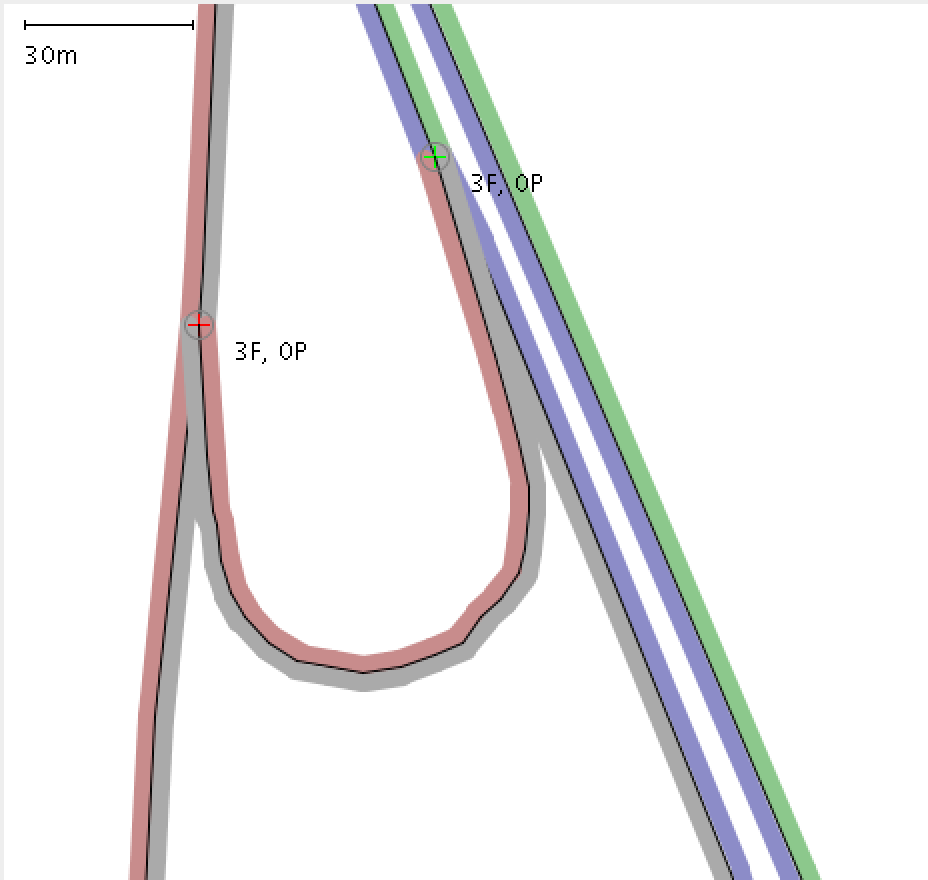
\includegraphics[width=0.4\textwidth]{figs/road/road_polyline.png}
            \hspace{0.2em}
            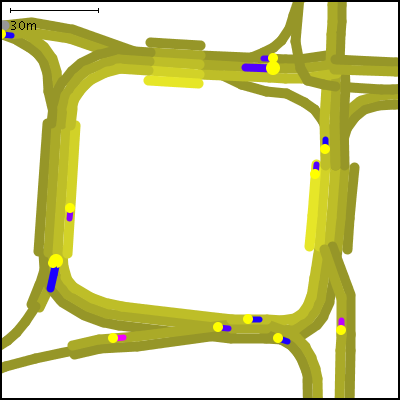
\includegraphics[width=0.4\textwidth]{figs/road/road_lanes.png}
        \end{figure}

        \item OSM xml import - as an XML file with published standard \(lane directions and such\)
            \begin{figure}[h]
                \caption{Process of preparing the OSM xml file using OSM tools}
                \label{fig:thirdPartyToolsOSMPreparation}
                \centering
                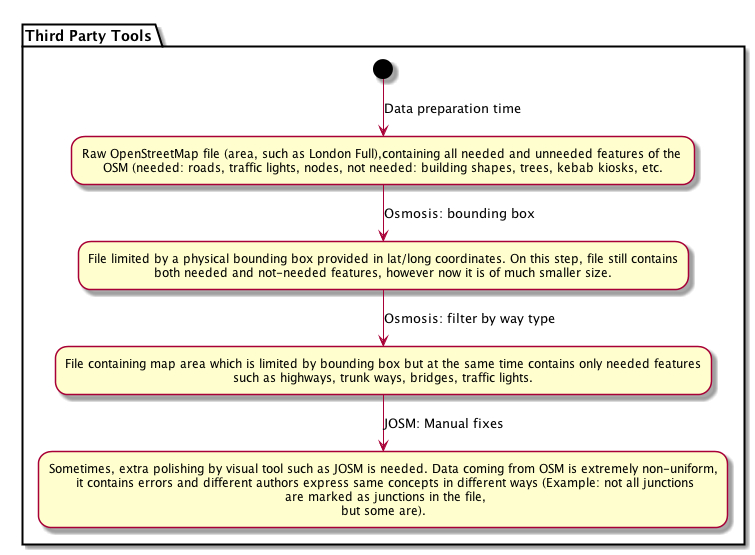
\includegraphics[width=0.8\textwidth]{../../uml_diagrams/thirdPartyToolsDataLoading.png}
            \end{figure}

        \item Types of data not working for us - we need  a connected graph of roads, OSM has some ways/nodes, loosely  connected \(via IDs\)
        \item Roads are represented as no-width polylines \(no individual lanes except for just having the property\). Such roads ar displayed in Figure \ref{fig:roadAndLanesPolylines}, on the left - original road polyline coming from OpenStreetMap XML file \(think black line\). On the right - typical example of result of lane generation.
        \item crossroads are sometimes marked nodes, sometimes just a node used in two ways.
        \item mention specifically the issue with the loosely coupled data/inaccurate data (human error, multiple representations etc.). We had to 'cut edges' to get it there.
        \item SUMO has that capability but implements its own tags and does some guess work
    \end{itemize}
\end{itemize}

\subsection{Graph construction}

\begin{itemize}
	\item Thoughts
    \begin{itemize}
        \item why construct the graph prior to the sim run instead of during
        \item > moving the workload at startup time so as to increase runtime performance
        \item > able to conceptually save state of graph on each tick if save is implemented
    \end{itemize}
    \item Graph constructed from description value objects of roads, junctions and links
    \item Original premise: Links, Junctions and Roads
    \item >Features (Roads and Junctions) are connected via links (still in high abstraction) see Figure~\ref{fig:FeatureConnect}

    \begin{figure}[h]
        \vspace{1.5em}
        \caption{Original design with Features and Links}
        \label{fig:FeatureConnect}
        \centering
        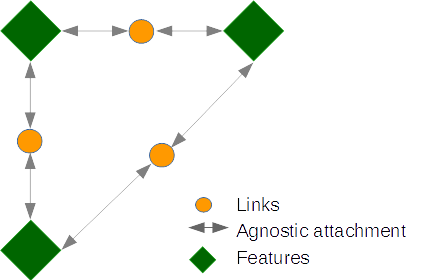
\includegraphics[width=0.50\textwidth]{figs/graphConstruction/OriginalConnections.png}
        \vspace{1.5em}
    \end{figure}

    \begin{figure}[h]
        \vspace{1.5em}
        \caption{Roads in the original high abstraction design}
        \label{fig:RoadsOriginal}
        \centering
        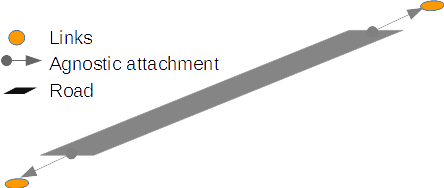
\includegraphics[width=0.45\textwidth]{figs/graphConstruction/OriginalRoads.png}
        \vspace{1.5em}
    \end{figure}

	\item Progressed into Links, Junctions, Lanes in Directed lane group in Road
	\item > linkage done on a lane level instead of road to make it easier to construct a directed graph, whilst maintaining access to groups of lanes and the road they belong to for traffic behaviour.
	\item >>>Example!
	\item link descriptions are depreciated after work on the OSM showed that universal linkage with junctions were for easier to do then identifying what was 1-to-1 link or a junction from the OSM data
	\item Graph now composed of directed lanes -> links and Junction features with special JunctionLinks
	\item Roads are now abstracted in the graph. Lanes still belong to groups of directed lanes which, in turn, belong to roads but the graph connections are done at lane level.
	
\begin{figure}[h]
	\vspace{1.5em}
  	\caption{Roads, Directed lane group and lanes}
  	\label{fig:RoadsFinal}
  	\centering
	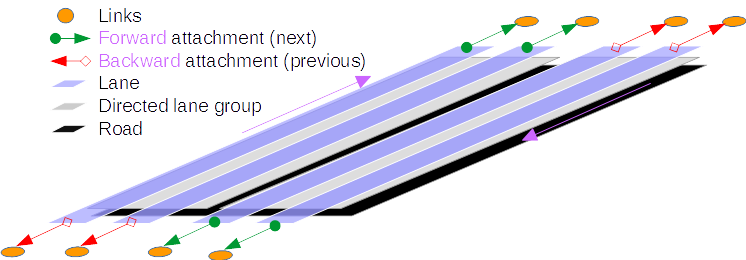
\includegraphics[width=0.75\textwidth]{figs/graphConstruction/Roads.png}
  	\vspace{1.5em}
\end{figure}	
	
\begin{figure}[h]
	\vspace{1.5em}
  	\caption{Junction}
  	\label{fig:junction}
  	\centering
	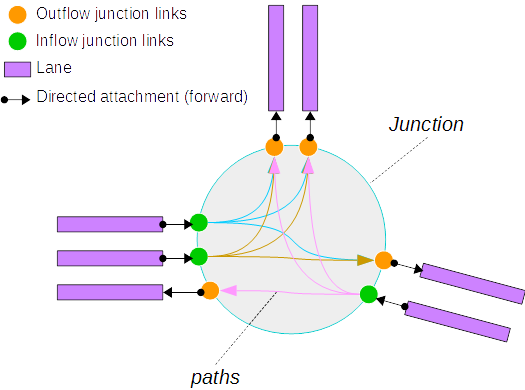
\includegraphics[width=0.6\textwidth]{figs/graphConstruction/Junction.png}
  	\vspace{1.5em}
\end{figure}
	
	\item Roads and directed lane kept for keeping track of what belongs where on the simulation map. e.g.: road with name can be back referenced from a lane.
	\item 
\end{itemize}

\begin{itemize}
	\item Problems:
	\item > issues streaming from the OSM data leads to bug where in a round about a incoming road cannot be connected up
	\item > Example!! + PIC + explanation as to why exactly
\end{itemize}

\subsection{Traffic Generators}
\begin{itemize}
	\item TF originally used to produce traffic only
	\item progressed to also receive traffic exiting the boundaries of the graph. Additional movement check - cars don't disappear anywhere but in Traffic Generators so we are sure on graph consistency at least in long run time.
	\item keeps tab on vehicles received and produced
	\item responsible for the destruction of vehicle object
	\item Bug: incoming only lanes to a junction
	\item Bug: 1 dual way road and then all incoming composed roads into junction meant that for the incoming of the 2 way road, the traffic had no where to go.
	\item >> Both dealt with by placing TF on junctions
	\item Bug: originally linkage was checked forward only in the direction of the lanes. Not backwards. meaning if no forward lanes were present in an asymmetric road then the outgoing lanes would not get a TF connected as they were not detected.
	\item Problem fixed by introducing the "previous link" connection to all features.
	\item Good for spotting OSM data issues/inconsistencies at a glance since the visualisation has TFs included on the map
	\item acts as a safety net for those (above)
	\item also, adding TFs during map construction ensures that 'island' features sets are not left without traffic on them
	\item *island: disconnected groups from the main graph or orphan features that either indicate error/inconsistencies in the OSM import data or physical islands on maps
	\item e.g.: 
	
\begin{figure}[h]
	\vspace{1.5em}
  	\caption{Island problem resolution}
  	\label{fig:islandReal}
  	\centering
	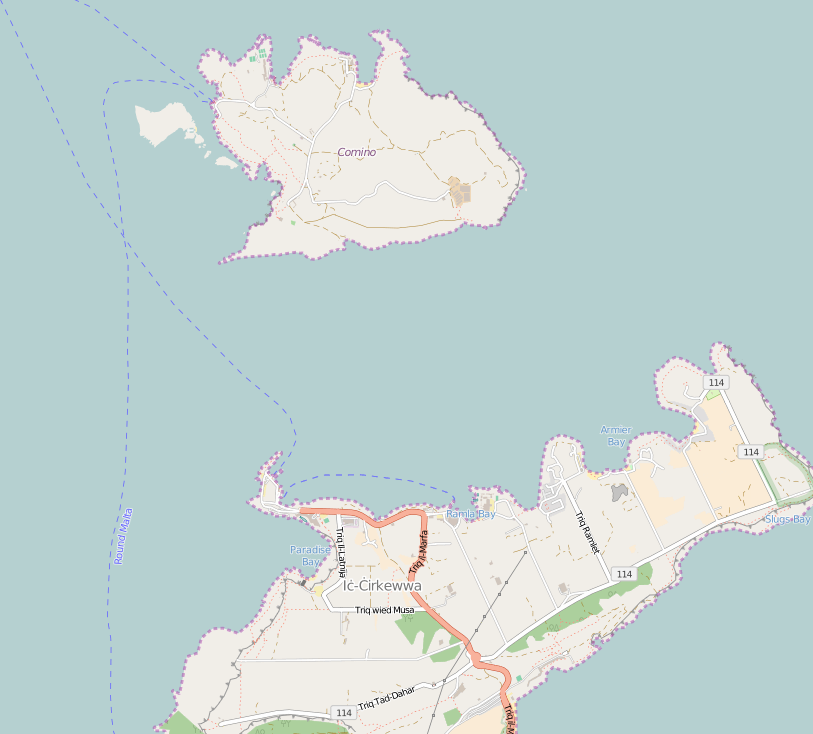
\includegraphics[width=0.4\textwidth]{figs/trafficGenerator/IslandExample_realmap.png}
	\hspace{0.2em}
	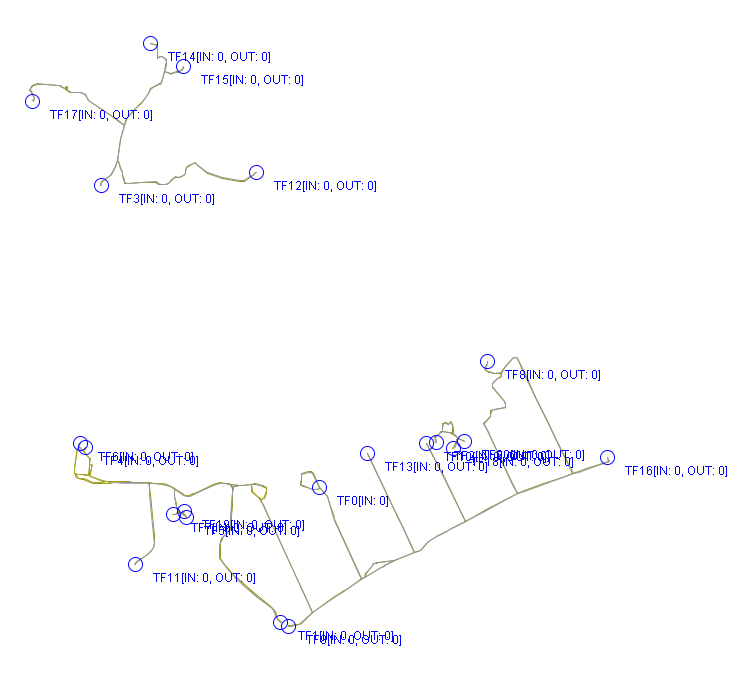
\includegraphics[width=0.40\textwidth]{figs/trafficGenerator/IslandExample_simmap.png}
  	\vspace{1.5em}
\end{figure}

\end{itemize}


\subsection{Traffic Lights}
\begin{itemize}
    \item two types of traffic lights: singles and those in one junction set
    \item all traffic lights work autonomously
	\item traffic light state: discussion whether traffic light State should be boolean or enum \(everyone wrote his version of boolean traffic lights, different ideas so we have taken Enum\)
\end{itemize}

\begin{itemize}
        \item traffic lights rules are basic, they do not change states according to the traffic (not intelligent traffic lights)
        \item only two states in traffic lights: red and green, we do not have early/late yellow etc.
\end{itemize}
     
\begin{itemize}
	\item serialization/de-serialization
\end{itemize}


\subsection{Map visualisation}
\begin{itemize}
    \item Map visualisation
    \begin{itemize}
        \item Coordinate conversion - lat/lon to meters-offset (Mercator projection). This is internal representaiton which is used in in simulation itself
        \item Coordinate conversion - meters-offset to pixels x/y (on-screen). This is the view-centric coordinate system which depends on scale, movement, size of window.
        \item Vehicle specific coordinates: lane it belongs to AND position along the polyline.
        \item GUI features: map zoom, pan, scale.
            \begin{figure}[h]
                \vspace{1.5em}
                \caption{Map zoom options}
                \label{fig:mapZoomOptions}
                \centering
                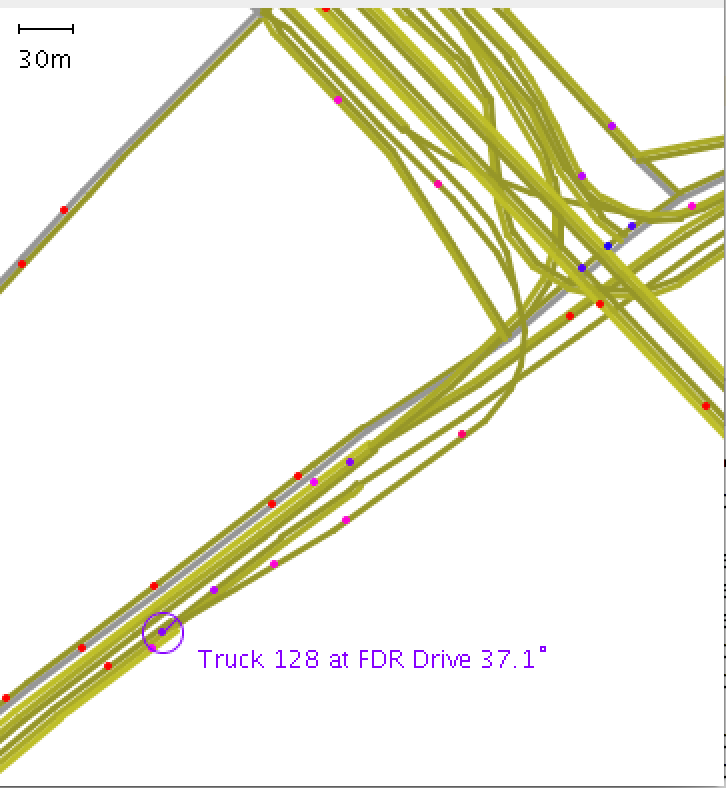
\includegraphics[width=0.4\textwidth]{figs/road/zoom_dots.png}
                \hspace{0.2em}
                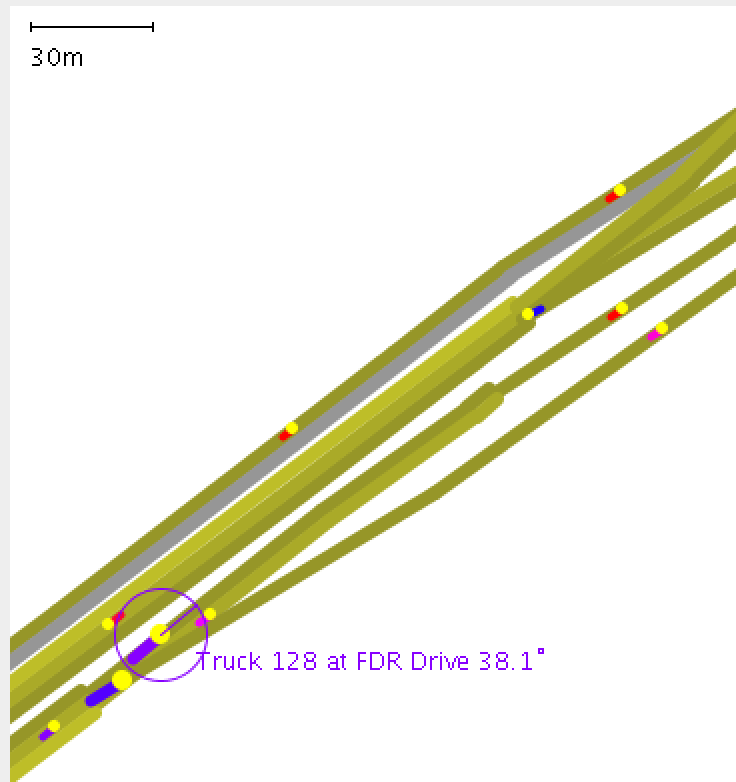
\includegraphics[width=0.4\textwidth]{figs/road/zoom_cars.png}
            \end{figure}

    \end{itemize}
\end{itemize}

\subsection{Vehicle movement}
\begin{itemize}
    \item Junctions and possible outcomes for vehicle
        \begin{figure}[h]
            \caption{Junctions found in real life}
            \label{fig:junctionTypes}
            \centering
            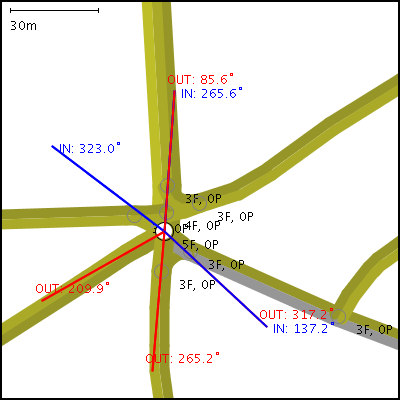
\includegraphics[width=0.4\textwidth]{figs/junction/junction_5_roads.png}
            \hspace{0.2em}
            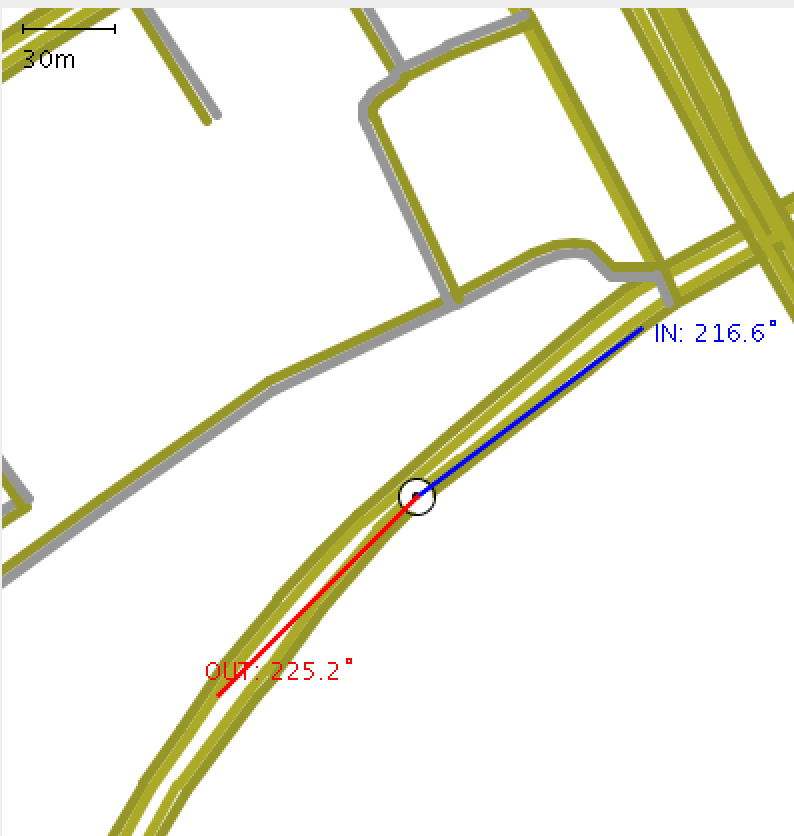
\includegraphics[width=0.4\textwidth]{figs/junction/junction_two_roads.png}
        \end{figure}

        \begin{figure}[h]
            \caption{Types of forks found in real life }
            \label{fig:forkTypes}
            \centering
            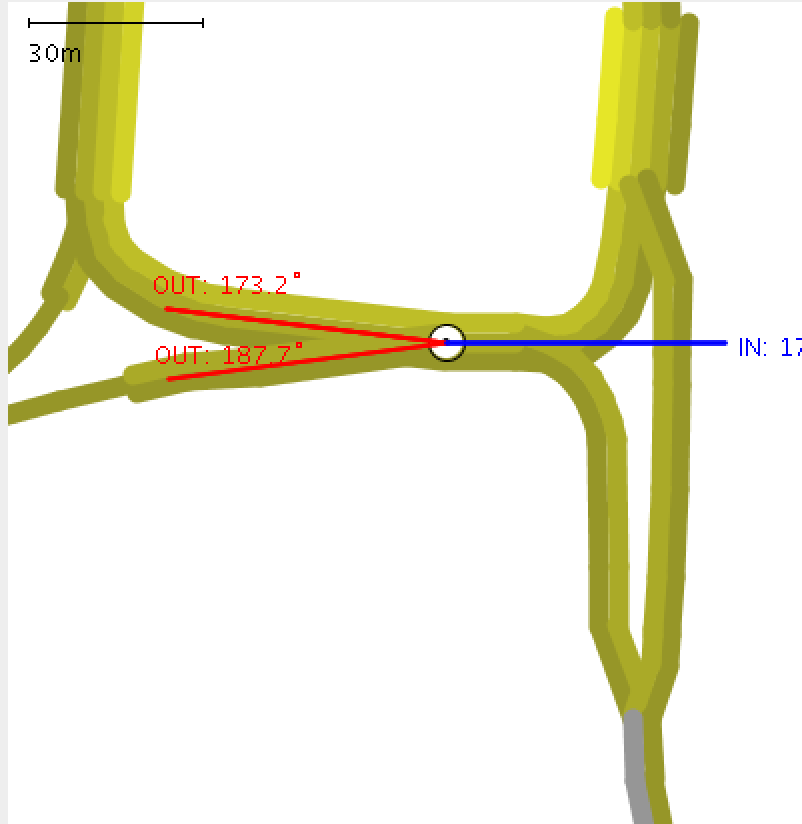
\includegraphics[width=0.4\textwidth]{figs/junction/junction_oneway_to_fork.png}
            \hspace{0.2em}
            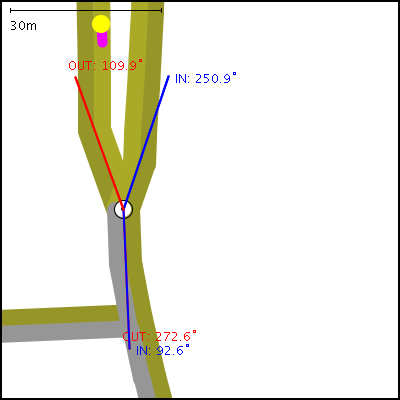
\includegraphics[width=0.4\textwidth]{figs/junction/junction_two_way_to_fork.png}
        \end{figure}

    \begin {itemize}
        \item our model: junctions 1-type: only 2 roads connected
        \item our model: junction 2-type: more than 2 roads connected (actual junctions)
            \begin{figure}[h]
                \caption{Junction forward or turn options depending on angle }
                \label{fig:forwardOrTurnOption}
                \centering
                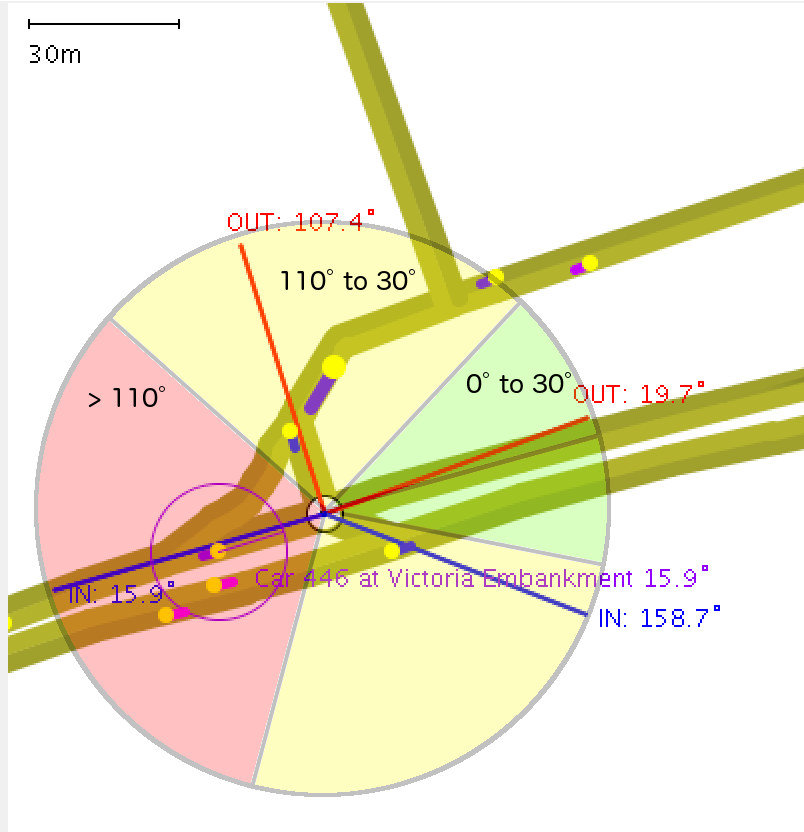
\includegraphics[width=0.4\textwidth]{figs/junction/junction_car_incoming_angle_with_turn_sectors.png}
            \end{figure}
        \item explain incoming lane angle, outgoing angles and its effect on vehicle movement - what is considered straight movement, and what is considered turn. >110 is prohibited, 110-30 is turn 30-0 is straight. This enforces us to skip weird turns at forks, for example.
    \end {itemize}

    \item Vehicle movement
        \begin{figure}[h]
            \caption{Car changing lane}
            \label{fig:carKeepingDistance}
            \centering
            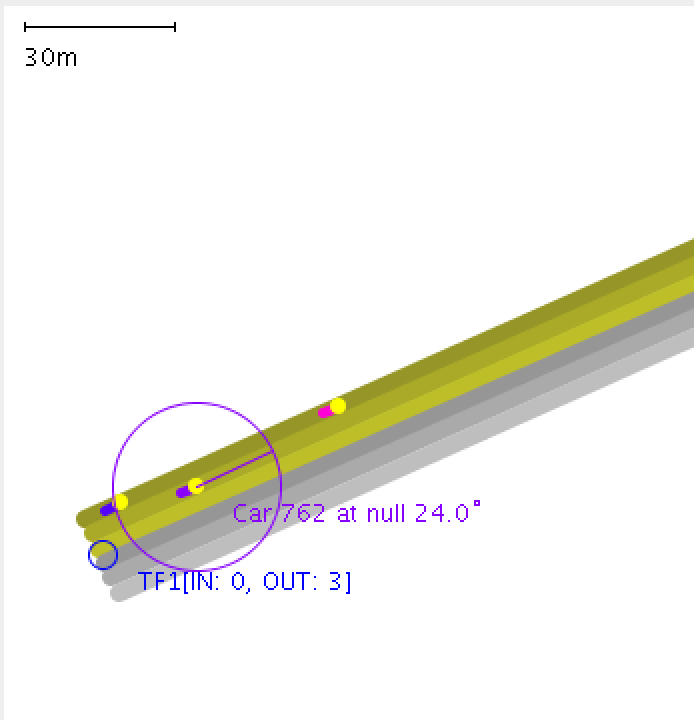
\includegraphics[width=0.3\textwidth]{figs/carMovement/car_keeping_distance_to_other.png}
            \hspace{0.2em}
            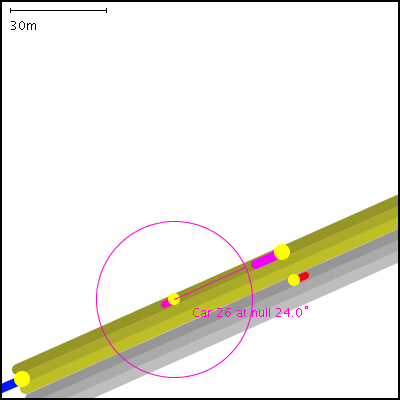
\includegraphics[width=0.3\textwidth]{figs/carMovement/car_lane_change_before.png}
            \hspace{0.2em}
            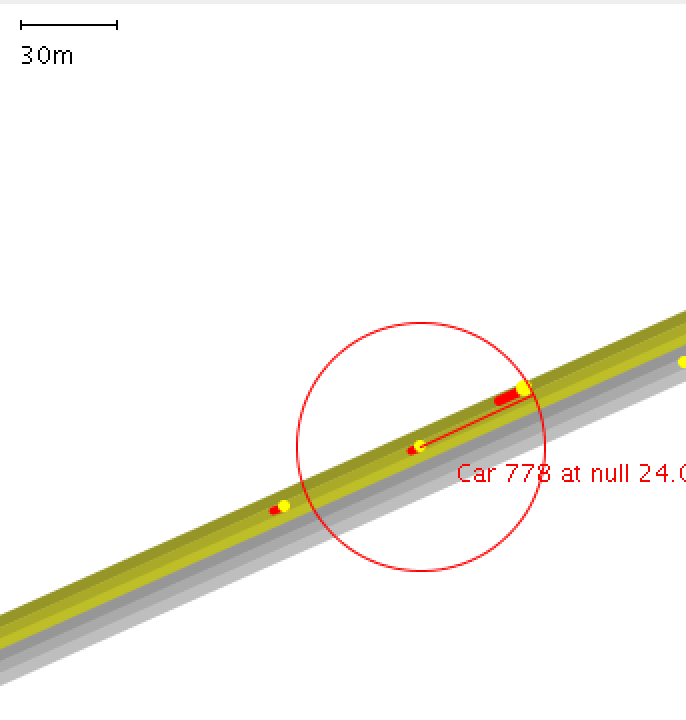
\includegraphics[width=0.3\textwidth]{figs/carMovement/car_lane_change_after.png}
        \end{figure}

    \begin{itemize}
        \item Straight movement on the road (even when curved). Acceleration and deceleration.
        \item Deciding if to go forward or turn (random)
        \item Crossings. Movement on 2+F crossroads (more than 2 features).
        \item Distance the car keeps to obstacles
        \item Lane changing - if there is another car in distance to keep, see to outer lane (if the same space is free) and change if possible, then try to do same for inner lane. If both buys, just brake.
    \end{itemize}

\end{itemize}


\subsection{Logger}
\begin{figure}[h]
	\vspace{1.5em}
  	\caption{Logger overview}
  	\label{fig:logger_overview}
  	\centering
	\includegraphics[width=0.75\textwidth]{figs/logger/LogModuleObjectDiagram.png}
  	\vspace{1.5em}
\end{figure}

\begin{itemize}
    \item explain why and usage scenarios
    \item > Debugging (1/3 resources for tracking down issues: exception, log, inline print)
    \item > Keep track of what's happening and have a non-volatile record of states during a particular run (for hard to reproduce errors)
    \item > custom 'homebrew' logger as only relatively simple logging required
    \item interface for logger included to that in the future another implementation or different logger can be used without too much trouble
    \item add basic arch. UML here
    \item Log config option injection \(why/how\)
    \item >Ability to inject log configuration options without recompiling the application
    \item >More flexible than hard coded options
    \begin{itemize}
    	\item Log levels
    	\item Output format (txt, csv, console)
    	\item Output name (file name in the case of txt and csv)
    	\item Exceptions in log switch
    	\item if no config file is found a default one is created that includes some guidelines on what options are available
    \end{itemize}
    \item Output formats (impact on performance)
    \item >text and csv will heavily influence runtime performance due to the lower performance of writing to files compared to memory
    \item txt for general record keeping
    \item csv useful for filtering data inside a spreadsheet software or importing to database - more flexible for reformatting the output also
    \item >console
    \item information recorded
    \begin{itemize}
    	\item Session message number
    	\item Date/Time stamp
    	\item message origin (class name usually)
\begin{lstlisting}[language=java]
	private static Logger_Interface LOG = Logger.getLoggerInstance(Road.class.getSimpleName());
\end{lstlisting}
    	\item NORMAL MSG
		\item message level (Fatal, error, normal msg, debug, trace)
    	\item EXCEPTIONS
    	\item stack trace of the exception
    \end{itemize}
    \item Since in Java most types are children of the Object class and we have autoboxing \cite{Oracle1995} for primitive types we can use 'Object' as the type for the signature of the method that are called to pass a message
    \item Log message passed through to log via arbitrary number of parameters
    \item '...' also known as 'vararg' \cite{Oracle2004}
\begin{lstlisting}[language=Java]
	void log_Error(Object... objects);
\end{lstlisting}   
	\item this allows easy message compositions with dynamic variables within. e.g.:
\begin{lstlisting}[language=Java]
	LOG.log_Error("Road '", lanes.getRoad().getID(), "' has group of directed lanes with partly implemented Links (Back). ", link_count, "/", lanes.getNumberOfLanes(), " Lanes connected to a link.");
	LOG.log_Trace("X--> '", lanes.getID(), "' has no previous link(s).");
\end{lstlisting} 

\end{itemize}


\section{Team Work}
%Describe how you worked together, including the tools and processes you used to facilitate group work.

\begin{itemize}
    \item learned how to properly use team-collaborative tools
    \begin{itemize}
            \item IntelliJ Idea
            \item >facilitated git work through their embedded VCS module
            \item >Very nice code/doc and test outline generation. Enables user to focus on the important stuff instead of boilerplate code
            \item Trello
            \item >Originally used to help with Kanban process but as the updates inside and usage were sporadic and only done by some members of the group it didn't live up to its fullest potential.
            \item Hipchat
            \item > Useful for day to day communication and updates with the github/trello plug-in to keep an overview on the activities done within the group
            \item > Not everyone was diligent in being on it whilst working on the code but, when used, very useful to shout out and get quick answers to question to the members online at the time.
     \end{itemize}

    \item learned time-allocating in collaborative environment
    \item learned  problem solving in collaborative environment
    \item learned  conflict solving in collaborative environment
    \item NOTE> Maybe worth talking about the group marking here once that's done.
    \item Regular weekly meetings
    \item learning from each other
    \item > (JUnit tests)
    \item > Technical problems addressed - Example?
    \item > Individual strengths can be shared in a group setting
\end {itemize}

Problems:
\begin{itemize}
    \item procrastination and lack of pro-activity were a problem.
    \item Extended periods of low output for the project lead to loosing track of the changes and difficulty understanding current states of the project on a technical level for some members
    \item Other peripheral tasks (both technical and not - e.g. research, docs, report.. ) tended to be ignored or relegated to the low priority list in cases
    \item code review was not as effective as it could have been in fostering legacy learning from more experienced members due to the sporadic contribution in cases
    \item In meetings: Code writing once the issues of the week were discussed was not as productive as it could have been during these sessions
    \item combination of these issues lead to an asymmetric distribution of work input on the project
\end{itemize}

\section{Evaluation}
%Critically evaluate your project: what worked well, and what didn’t? How did you do relative to your plan? what changes were the result of improved thinking and what changes were forced upon you? how did your team work together? etc. Note that you need to show that you understand the weaknesses in your work as well as its strengths. You may wish to identify relevant future work that could be done on your project.
\subsection{Possible further development}
\begin{itemize}
	\item Scaling number of cars to the size of the graph  (map)
	\item Round about issue with importing OSM data made by humans 
	\item -> allow export from other sources /API calls (gmap?)
	\item -> allow for manual editing of the graph from the GUI view?
	\item As skirting into hybrid model, detailing such as car sprites, road graphics, etc could be added as zoom factor increases, maybe show lanes from medium zoom and abstract into dots and coloured roads at low zoom
	\item addition of plug-in capability to add different metrics/behaviours as required by the user
	\item creation of vehicles with specs based off real life data
	\item >pollution based on vehicle profile
	\item manual addition of temporary block on map so modify traffic flow (construction/road works/accidents/etc..)
	\item Simulation recorder/player - large simulations can be run prior then played and analysed later
	\item NOTE: Traffic lights??
\end{itemize}

\begin{itemize}
    \item Log module expansion
    \begin{itemize}
        \item coloured terminal window if more time,
        \item >easier to read
        \item >segregated from the console
        \item Custom Filters
        \item >filtering based on class name (origin)
        \item >filtering based on selection of multiple non-sequential log levels instead of everything below the set global level (granular control)
    \end{itemize}
\end{itemize}

\subsection{Performance}
After the implementation of main application, performance measurements were taken.

\begin{itemize}
    \item Measurements: what are we measuring.
    \item Method: just one sample, since the time is constant and independent, cold JVM, measurement using System.currentTimeMillis() on entrance and exit to corresponding method.
    \item Results are provided in Table \ref{table:performanceComparison}
    \item Test machine: OS X, Intel Core I7-4770HQ, 2.2 GHz, 16GB RAM, SSD
\end{itemize}



\begin{center}
\begin{longtabu} to \textwidth {|
    X[2,l]|
    X[4,l]|
    X[3,c]|
    X[3,c]|
    X[3,c]|
    }
    \hline
    \textbf{Sample} & \textbf{Size} & \textbf{XML load} & \textbf{Graph linkage} & \textbf{Roads draw time} \\ \hline
Straight road & 1 road and 0 junction, 9 mapFeatures, 12 mapLinks, 2 traffic generators & 4 & 0 & 2 \\ \hline
Elephant and Castle & 101 road and 80 junction, 454 mapFeatures, 18 mapLinks, 12 traffic generators & 37 & 4 & 8 \\ \hline
Paris, Arc & 284 road and 168 junction, 1145 mapFeatures, 57 mapLinks, 35 traffic generators & 118 & 68 & 70 \\ \hline
Manhattan, Battery Park & 212 road and 148 junction, 829 mapFeatures, 81 mapLinks, 40 traffic generators & 11 & 5 & 29 \\ \hline
Strand area & 781 road and 530 junction, 2998 mapFeatures, 196 mapLinks, 105 traffic generators & 62 & 19 & 41 \\ \hline
Buckingham Palace& 275 road and 176 junction, 1032 mapFeatures, 68 mapLinks, 41 traffic generators & 28 & 8 & 21 \\ \hline
Whole Manhattan & 14763 road and 10429 junction, 58394 mapFeatures, 1055 mapLinks, 596 traffic generators & 13607 & 468 & 531 \\ \hline
Whole Greater London & 31101 road and 24314 junction, 120672 mapFeatures, 547 mapLinks, 391 traffic generators & 32911 & 644 & 1087 \\ \hline

\caption{Load and render times for different map samples}
\label{table:performanceComparison}
\end{longtabu}
\end{center}


\section{Peer Assessment}
%In a simple table, allocate the 100 ‘points’ you are given to each team member. Valid values range from 0 to 100 inclusive. You may assign decimal values, but the entire points must add up to precisely 100.

 \begin{itemize}
        \item Kumar Awijeet
		\item Oleksandr Cherednychenko
		\item Esmond A. Davison
		\item Jacek Krupski
		\item Farhad Rahimli
    \end{itemize}

\section{Git log details}
Following are name to Git alias mappings:

\begin{itemize}
   \item Esmond Davison: E. A. Davison, Es, E A. Davison
   \item Farhad Rahimli: dlphi
   \item Kumar Awijeet: kumar awijeet
   \item Oleksandr Cherednychenko: Oleksandr Cherednychenko,  Alexander Cherednichenko
\end{itemize}
\begin{center}
\begin{longtabu} to \textwidth {|
    X[3,l]|
    X[2,c]|
    X[8,l]|}
    \hline
    \textbf{Author} & \textbf{Date} & \textbf{Message} \\ \hline
Alexander Cherednichenko & 2016-01-20 & Initial commit \\ \hline
Oleksandr Cherednychenko & 2016-01-21 & Adding reports structure, ignores and some seeds for READMEs \\ \hline
E A. Davison & 2016-01-22 & Basic LaTEX files and preamble \\ \hline
Oleksandr Cherednychenko & 2016-01-22 & Correcting ignores for LaTeX \\ \hline
dlphi & 2016-01-25 & test by farik \\ \hline
dlphi & 2016-01-26 & changes to readme \\ \hline
Oleksandr Cherednychenko & 2016-01-26 & Adding corrected gitignore for IntelliJ IDEA not to commit project files (we will use gradle or maven for POM) \\ \hline
E A. Davison & 2016-01-26 & Examples of list, enumeration and the 3 basic types of headings for some starting up help. \\ \hline
Oleksandr Cherednychenko & 2016-01-27 & Adding a build system to the branch, with minimalistic Gradle build. We have 2 submodules, and a top-level gradle build. During the build tests are run (JUnit, Mockito for now), and the result is packaged into runnable apps (/bin and /lib substructure with OS-specific scripts). Modified ther README to reflect all these changes. \\ \hline
Oleksandr Cherednychenko & 2016-01-27 & Added fest-assert for quick and fluent assertions. Updated README \\ \hline
E A. Davison & 2016-01-29 & Quick outline with some basic points added for preliminary report with the report requirements copy-pasted for everyone's convenience \\ \hline
Oleksandr Cherednychenko & 2016-01-29 & Expanded the items for the initial report - mostly what is that we plan to go building \\ \hline
dlphi & 2016-01-31 & adding one bullet point \\ \hline
dlphi & 2016-01-31 & Merge remote-tracking branch 'origin/master' \\ \hline
Inspiron17R & 2016-01-31 & Simulation engine introduction \\ \hline
E A. Davison & 2016-02-01 & Log module (basic) preliminary commit \\ \hline
E A. Davison & 2016-02-01 & Added *.class to the ignore list \\ \hline
E A. Davison & 2016-02-01 & Deleted <Log-Formatter> as functionality migrated to Output specific formatters \\ \hline
Oleksandr Cherednychenko & 2016-02-01 & Removing obsolete settings.gradle from both the subprojects. \\ \hline
Oleksandr Cherednychenko & 2016-02-01 & Adding structure for Es's log module, with dependencies \\ \hline
E A. Davison & 2016-02-01 & PlantUML file for the Class Diagram of the logging system (not complete) \\ \hline
E A. Davison & 2016-02-01 & v.light editing on report \\ \hline
Oleksandr Cherednychenko & 2016-02-01 & Adding basic class diagram to start talking about simulation \\ \hline
E A. Davison & 2016-02-01 & Some re-aranging in the Logger uml diagram \\ \hline
Inspiron17R & 2016-02-02 & Engine report -> technology view \\ \hline
Inspiron17R & 2016-02-02 & Initial report --> Engine's paragraph bibliography \\ \hline
E A. Davison & 2016-02-02 & Added FileIO class to Logger and updated UML class diag. to reflect that \\ \hline
Oleksandr Cherednychenko & 2016-02-02 & Merge branch 'master' into build-system \\ \hline
Oleksandr Cherednychenko & 2016-02-02 & Merge branch 'master' into build-system \\ \hline
Oleksandr Cherednychenko & 2016-02-02 & Moving log files into the new build structure according to packages. \\ \hline
dlphi & 2016-02-02 & Merge remote-tracking branch 'origin/master' \\ \hline
Oleksandr Cherednychenko & 2016-02-02 & Updating readme on how to get the project up and running. \\ \hline
Oleksandr Cherednychenko & 2016-02-02 & Fixing readme formatting \\ \hline
E A. Davison & 2016-02-02 & Moved Logger uml diagram files \\ \hline
E A. Davison & 2016-02-02 & Report: stuff done in group session \\ \hline
Oleksandr Cherednychenko & 2016-02-03 & Expanded 2nd part of the initial report: the process. \\ \hline
Oleksandr Cherednychenko & 2016-02-03 & Added overall architecture diagram \\ \hline
E A. Davison & 2016-02-03 & 1st part of initial report \\ \hline
E A. Davison & 2016-02-03 & Merge branch 'master' of https://github.com/teamIndexZero/index-zero-trafficsystem \\ \hline
E A. Davison & 2016-02-03 & report architecture diagram added to figs \\ \hline
E A. Davison & 2016-02-03 & renamed package to convention (lowercase) \\ \hline
Oleksandr Cherednychenko & 2016-02-03 & Finished initial part 2 of the report. \\ \hline
E A. Davison & 2016-02-03 & log.fileIO.FileIO class implemented + uml diagram updated \\ \hline
E A. Davison & 2016-02-03 & Light editing on preliminary project report (some wording and spacing) \\ \hline
E A. Davison & 2016-02-04 & Group edits on intermediate report \\ \hline
kumar awijeet & 2016-02-04 & PPT for intial report \\ \hline
E A. Davison & 2016-02-04 & log.fileio.FileIO decomposition into FileIO and FileInput/FileOutput classes \\ \hline
E A. Davison & 2016-02-04 & Merge branch 'master' of https://github.com/teamIndexZero/index-zero-trafficsystem \\ \hline
E A. Davison & 2016-02-06 & Debugging, added Output-TXT functionalities, added a MicroLogger for lightweight logging functionality for the Log module (avoids infinite loop/stack overflow when Logger is used on itself) \\ \hline
E A. Davison & 2016-02-07 & Added toString method to Log-TimeStamp \\ \hline
E A. Davison & 2016-02-07 & Added javadoc descriptions to MicroLogger class \\ \hline
kumar awijeet & 2016-02-07 & PPT for initial report \\ \hline
E A. Davison & 2016-02-07 & Log-TimeStamp bug where test would sometimes fail during certain periods of the day squashed (hopefully). \\ \hline
E A. Davison & 2016-02-07 & Added preliminary log-Exception( Exception e ) interface and functionality to Logger \\ \hline
Oleksandr Cherednychenko & 2016-02-07 & Added jacoco for coverage. Fixed global scope for the jUnit - we now can test on top-level module. \\ \hline
E A. Davison & 2016-02-07 & Updated Gradle options to include the Jacoco test coverage plug-in \\ \hline
E A. Davison & 2016-02-07 & Merge branch 'master' of https://github.com/teamIndexZero/index-zero-trafficsystem \\ \hline
E A. Davison & 2016-02-07 & Output and Formatter for the CSV implemented \\ \hline
Oleksandr Cherednychenko & 2016-02-07 & Added more ignores for logs \\ \hline
E A. Davison & 2016-02-07 & Some clean up of the Log-Config and beginning of implementation for the log configuration file loader/checker \\ \hline
E A. Davison & 2016-02-07 & Cleanup of FileInput's exceptions (now sending to MicroLogger), added the message number to exception all outputs/formatters so now shows properly, \\ \hline
Oleksandr Cherednychenko & 2016-02-07 & Added initial run of the simulation. Very basic, boolean 2-dimension array as a base for cell automata map, collection of objects, simplisic rendering. \\ \hline
kumar awijeet & 2016-02-08 & Updated PPT for initial report \\ \hline
E A. Davison & 2016-02-08 & Formatter-TXT and Formatter-TERM unit tests added \\ \hline
E A. Davison & 2016-02-08 & fileIO.Output unit test created \\ \hline
dlphi & 2016-02-08 & Merge remote-tracking branch 'origin/master' \\ \hline
E A. Davison & 2016-02-09 & Added clearFileContent() in log.fileIO.FileOutput, work done on implementation of the config loader in log.Log-Config \\ \hline
E A. Davison & 2016-02-09 & Added variable option (for the log level for now) to the default config writer and the matching regex to the checker \\ \hline
kumar awijeet & 2016-02-09 & PPT for initial report \\ \hline
Oleksandr Cherednychenko & 2016-02-09 & Improved simulation and a bit of gui. We now have colors for objects. Redone rendering - now instead of bitmap from map[] thing we have objects drawn one by one. \\ \hline
E. A. Davison & 2016-02-09 & Bug squashed in log.fileIO.FileOutput where when clearing the file it would leave the state closed, log.Log-Config file loader for the config implemented \\ \hline
E. A. Davison & 2016-02-09 & Fixed typo in OutputTest \\ \hline
E. A. Davison & 2016-02-09 & Squashed bug that kept defaulting to default file name output for logs despite names being different in the config file, added a timestamp extension to all file outputs, added more examples to the default log-config file \\ \hline
dlphi & 2016-02-09 & Merge remote-tracking branch 'origin/master' \\ \hline
kumar awijeet & 2016-02-10 & Replacing old file - orignal method not working. Trying another process. \\ \hline
kumar awijeet & 2016-02-10 & Final PPT files for intial report \\ \hline
E. A. Davison & 2016-02-11 & Final report headings added and section info from the guidelines added in as comments \\ \hline
Oleksandr Cherednychenko & 2016-02-11 & Added readme quick notes on Running the software. Ignored log-config.cfg \\ \hline
Oleksandr Cherednychenko & 2016-02-11 & Merge remote-tracking branch 'origin/master' \\ \hline
Oleksandr Cherednychenko & 2016-02-12 & Merge remote-tracking branch 'origin/farik' \\ \hline
E. A. Davison & 2016-02-12 & Activity diag for the basic demo added, folder for uml stuff created and all other uml diag migrated to it. \\ \hline
E. A. Davison & 2016-02-12 & Changed default log level to "WARNING" to keep logging light by default for performance (disk IO) -> if level need to be changed do it in the log-config.cfg file from now on. \\ \hline
Oleksandr Cherednychenko & 2016-02-12 & 1 of 2 Simulator Improvements - added quite a lot of comments mostly. \\ \hline
dlphi & 2016-02-12 & Merge remote-tracking branch 'origin/master' \\ \hline
Oleksandr Cherednychenko & 2016-02-12 & 2 of 2 Simulator improvements - added comments where appropriate \\ \hline
Oleksandr Cherednychenko & 2016-02-12 & Merge remote-tracking branch 'origin/master' into simulatorImprovements \\ \hline
Oleksandr Cherednychenko & 2016-02-12 & Merge. \\ \hline
Oleksandr Cherednychenko & 2016-02-12 & Updated class diagram to the actual state \\ \hline
Oleksandr Cherednychenko & 2016-02-12 & Updated class diagram to the actual state \\ \hline
E. A. Davison & 2016-02-12 & Cleaned out code in Log-Config: simplified loadConfiguration(..), applyConfigurationLine(..) now return boolean \\ \hline
Alexander Cherednichenko & 2016-02-12 & Merge pull request -2 from teamIndexZero/logImprovements \\ \hline
Es & 2016-02-12 & Merge pull request -1 from teamIndexZero/simulatorImprovements \\ \hline
Inspiron17R & 2016-02-13 & CrossRoads--> class first version, architecture. \\ \hline
Oleksandr Cherednychenko & 2016-02-13 & Emergency fix - commented out @Jacek's code which is breaking the build so that others can build master branch. \\ \hline
E. A. Davison & 2016-02-13 & log.Logger unit test (with mockito) \\ \hline
E. A. Davison & 2016-02-13 & Merge branch 'master' of https://github.com/teamIndexZero/index-zero-trafficsystem into logImprovements \\ \hline
Oleksandr Cherednychenko & 2016-02-13 & Added some basic tests for simulator - mostly making sure it runs the ISimulationAware instances in correct order. \\ \hline
Oleksandr Cherednychenko & 2016-02-13 & Trying to trigger travis build with this commit - amending the pull request. \\ \hline
Oleksandr Cherednychenko & 2016-02-13 & Adding travis build server description file \\ \hline
Oleksandr Cherednychenko & 2016-02-13 & Trying to force Travis to use jdk 8 (and language level 8) \\ \hline
Oleksandr Cherednychenko & 2016-02-13 & Fixing weird case bug - IDEA does not recognize file is in lower case \\ \hline
Oleksandr Cherednychenko & 2016-02-13 & Merge branch 'master' into simulatorImprovements \\ \hline
Inspiron17R & 2016-02-13 & CrossRoads-->adding mechanical and automatic lights. \\ \hline
Inspiron17R & 2016-02-13 & CrossRoads-->adding mechanical and automatic lights. \\ \hline
Inspiron17R & 2016-02-13 & Merge remote-tracking branch 'origin/master' \\ \hline
Inspiron17R & 2016-02-13 & CrossRoads-->adding mechanical and automatic lights. \\ \hline
Inspiron17R & 2016-02-14 & Vehicle2 --> temporary class. CrossRoads-->linking with Vehicle 2. \\ \hline
E. A. Davison & 2016-02-14 & Merge branch 'master' of https://github.com/teamIndexZero/index-zero-trafficsystem into logImprovements \\ \hline
dlphi & 2016-02-14 & Merge remote-tracking branch 'origin/master' \\ \hline
dlphi & 2016-02-14 & adding serialization (writing) to main method \\ \hline
dlphi & 2016-02-14 & adding Serializable \\ \hline
dlphi & 2016-02-14 & adding deserialization \\ \hline
Inspiron17R & 2016-02-15 & CrossRoads-->improvements. \\ \hline
E. A. Davison & 2016-02-15 & Merge branch 'simulatorImprovements' of https://github.com/teamIndexZero/index-zero-trafficsystem into logImprovements \\ \hline
E. A. Davison & 2016-02-15 & Merge branch 'serialization' of https://github.com/teamIndexZero/index-zero-trafficsystem into logImprovements \\ \hline
E. A. Davison & 2016-02-15 & Merge branch 'master' of https://github.com/teamIndexZero/index-zero-trafficsystem into logImprovements \\ \hline
E. A. Davison & 2016-02-15 & Small tweak in main classes to make them more testable + depreciation of unused method(s) in Log-Engine \\ \hline
Inspiron17R & 2016-02-16 & Straight cars movement on the crossroad. \\ \hline
E. A. Davison & 2016-02-16 & Merge branch 'master' of https://github.com/teamIndexZero/index-zero-trafficsystem into logImprovements \\ \hline
E. A. Davison & 2016-02-17 & Log-Engine unit tests implemented \\ \hline
E. A. Davison & 2016-02-17 & Log-Engine unit test implemented \\ \hline
E. A. Davison & 2016-02-17 & Log-Config unit tests implemented \\ \hline
E. A. Davison & 2016-02-17 & Output-TERM unit tests implemented \\ \hline
dlphi & 2016-02-17 & Merge remote-tracking branch 'origin/master' \\ \hline
Es & 2016-02-17 & Merge pull request -3 from teamIndexZero/simulatorImprovements \\ \hline
Oleksandr Cherednychenko & 2016-02-17 & Pusing the new branch for movement, features and traffic lights. \\ \hline
dlphi & 2016-02-17 & some bullet points \\ \hline
dlphi & 2016-02-17 & Merge remote-tracking branch 'origin/master' \\ \hline
Oleksandr Cherednychenko & 2016-02-17 & Merge remote-tracking branch 'origin/master' into graphAndMovement \\ \hline
E. A. Davison & 2016-02-17 & Output-TXT unit tests implemented + some changes to FileIO/FileOutput and Output-TXT to ease testing \\ \hline
E. A. Davison & 2016-02-17 & FileIO unit tests implemented + minor corrections to Log code \\ \hline
E. A. Davison & 2016-02-17 & Revert "Merge branch 'serialization' of https://github.com/teamIndexZero/index-zero-trafficsystem into logImprovements" \\ \hline
E. A. Davison & 2016-02-17 & Unit test fail repairs (1/2) \\ \hline
E. A. Davison & 2016-02-17 & Unit test fail repairs (2/2) \\ \hline
E. A. Davison & 2016-02-17 & Formatter-CSV unit tests implementation (1/2) \\ \hline
E. A. Davison & 2016-02-18 & File-Output unit tests partly implemented.. (not fully successful) \\ \hline
E. A. Davison & 2016-02-19 & Deleted useless section of the Log-Config.getGlobalLevel() unti test \\ \hline
Oleksandr Cherednychenko & 2016-02-20 & Ignoring the test with missing functionality - it is described in TODO \\ \hline
Oleksandr Cherednychenko & 2016-02-21 & Moved things into corresponding packages. Added threading support to Simulator. Added toolbar to main window. \\ \hline
E. A. Davison & 2016-02-21 & File-Output unit tests implemented - working \\ \hline
Oleksandr Cherednychenko & 2016-02-21 & Merge branch 'master' into logImprovements \\ \hline
Alexander Cherednichenko & 2016-02-21 & Merge pull request -4 from teamIndexZero/logImprovements \\ \hline
E. A. Davison & 2016-02-21 & File-Input unit tests implemented + some added funct. to ease testing \\ \hline
E. A. Davison & 2016-02-21 & Merge remote-tracking branch 'origin/logImprovements' into logImprovements \\ \hline
E. A. Davison & 2016-02-21 & Beautification of msg number for TERM and TXT output + tests updated \\ \hline
E. A. Davison & 2016-02-21 & Output-CSV and Formatter-CSV with their test done + some minor corrections \\ \hline
Oleksandr Cherednychenko & 2016-02-21 & Addel GuiModel::Reset and proper painting lifeecycle for the map panel component. \\ \hline
Oleksandr Cherednychenko & 2016-02-21 & Getting coordinates to order \\ \hline
Oleksandr Cherednychenko & 2016-02-21 & Merge remote-tracking branch 'origin/master' into backgroundThread \\ \hline
Alexander Cherednichenko & 2016-02-21 & Merge pull request -5 from teamIndexZero/logImprovements \\ \hline
Oleksandr Cherednychenko & 2016-02-21 & Merge remote-tracking branch 'origin/master' into backgroundThread \\ \hline
Oleksandr Cherednychenko & 2016-02-22 & Added UML diagram for threading and MVC. \\ \hline
Oleksandr Cherednychenko & 2016-02-22 & Added tests for GUI controller Added commentaries to the code. \\ \hline
Oleksandr Cherednychenko & 2016-02-22 & Reformatting code and optimizing imports. \\ \hline
E. A. Davison & 2016-02-24 & File-Input/File-Output .close* updated with raising exception when failing instead of boolean \\ \hline
Inspiron17R & 2016-02-24 & Merge remote-tracking branch 'origin/master' into graphAndMovement \\ \hline
E. A. Davison & 2016-02-24 & Formatter-CSV - any ';' replaced with '¬' before csv formatting to avoid extra unwanted cols in output. Unit test updated with this in mind. \\ \hline
Alexander Cherednichenko & 2016-02-24 & Merge pull request -6 from teamIndexZero/logImprovements \\ \hline
Oleksandr Cherednychenko & 2016-02-24 & Merge remote-tracking branch 'origin/master' into backgroundThread \\ \hline
Oleksandr Cherednychenko & 2016-02-24 & Fixing the reset test. \\ \hline
Es & 2016-02-24 & Merge pull request -7 from teamIndexZero/backgroundThread \\ \hline
Oleksandr Cherednychenko & 2016-02-25 & Merge branch 'master' into graphAndMovement \\ \hline
Oleksandr Cherednychenko & 2016-02-25 & Resolving textual conflicts after the changes were merged in. \\ \hline
Inspiron17R & 2016-02-26 & Merge branch 'graphAndMovement' of https://github.com/teamIndexZero/index-zero-trafficsystem into graphAndMovement \\ \hline
Inspiron17R & 2016-02-27 & Movement improvements. \\ \hline
Inspiron17R & 2016-02-27 & Movement improvements adding lines class. \\ \hline
E. A. Davison & 2016-02-27 & Graph creation beginnings... (+fresh start of the features/links for e-z preliminary testing) \\ \hline
E. A. Davison & 2016-02-27 & ongoing work save... resuming tomorrow \\ \hline
E. A. Davison & 2016-02-28 & SimulationMap modified to enable feature/link injection through constructor \\ \hline
E. A. Davison & 2016-02-28 & Final Report update (some Log module stuff and mention of OSM and SUMO (<-need expansion) ) \\ \hline
E. A. Davison & 2016-02-28 & Save point (work in progress) \\ \hline
E. A. Davison & 2016-02-28 & Save point (work in progress) \\ \hline
E. A. Davison & 2016-02-28 & Save point (work in progress) \\ \hline
E. A. Davison & 2016-03-01 & Save point (work in progress) - Feature[Road/DirectedLanes/Lane/RoadSpecs], ID augmented with descriminant constructor, some class moved into their own packages (i.e. cleaning up) \\ \hline
E. A. Davison & 2016-03-01 & Unit Tests for: DirectedLanes, Lane, ID + small mods to squash found bugs \\ \hline
E. A. Davison & 2016-03-01 & Unit Test: Road + some changes to the class to add getLeftLaneCount and getRightLaneCount methods \\ \hline
E. A. Davison & 2016-03-01 & Save point (work in progress) - GraphConstructor created to move that concern out of the SimulationMap. LinkDescription added for carrying description of the logical connections inside the graph to the GraphConstructor. \\ \hline
E. A. Davison & 2016-03-01 & Save point (work in progress) - More work on the GraphConstructor, added ID for the LinkDescription class and a LinkType class. \\ \hline
E. A. Davison & 2016-03-01 & Save point (work in progress) - LinkDescription.toString() added + its Unit Test \\ \hline
E. A. Davison & 2016-03-01 & Save point (work in progress) - GraphConstructor.createGraph() now can deal with features that end abruptly. \\ \hline
E. A. Davison & 2016-03-01 & Save point (work in progress) - Link.isDeadEnd() method added \\ \hline
E. A. Davison & 2016-03-02 & Save point (work in progress) - GraphConstructor.addLink(..) done, MissingImplementationException class added for missing switch cases in the code, Basic traffic light classes added. \\ \hline
E. A. Davison & 2016-03-02 & Save point (work in progress) - Traffic light classes arranged, Road descriptor added \\ \hline
E. A. Davison & 2016-03-02 & Save point (work in progress) - TrafficLightRule \\ \hline
E. A. Davison & 2016-03-02 & simulator object diagram outline (not complete) \\ \hline
E. A. Davison & 2016-03-02 & simulator object diagram outline (not complete) edit. \\ \hline
E. A. Davison & 2016-03-02 & Save point \\ \hline
Oleksandr Cherednychenko & 2016-03-02 & Fixing the graph buildup (original) in order to carry on with coordinate system conversion. \\ \hline
E. A. Davison & 2016-03-02 & RoadLink (composed of Link(s)) added for linking macro Features like Road - Junction \\ \hline
Oleksandr Cherednychenko & 2016-03-03 & Added OSM loader (from XML). Added three sample OSM files - for Strand, El'n'castle, and for Buckingham palace area. Added a preliminary UI component - the app starts with the initial small screen where user can select their map (one of pre-set for now). Added proper coordinate conversion between lat/lon within the bounding box, and on-screen coordinate (for now it SCALES!) \\ \hline
Oleksandr Cherednychenko & 2016-03-03 & Minor fix for the interface. \\ \hline
Oleksandr Cherednychenko & 2016-03-03 & Refactoring window out to the extra class to make it a bit more readable. Decoupling the window size through model (no direct dependency between panel and imageproducer now). \\ \hline
E. A. Davison & 2016-03-04 & Work on the descriptors (added JunctionDescriptor class as place holder) \\ \hline
E. A. Davison & 2016-03-04 & Removed redundant comments \\ \hline
Oleksandr Cherednychenko & 2016-03-04 & Added coordinate conversion latlon -> geo Added UI for map list. Added UI for settings Added highlighting of the moving car. Added car details panel. Tweaked traffic generator. Tweaked traffic remover. Polyline roads - now, the road is represented by geo polyline, and movement happens along it. \\ \hline
Oleksandr Cherednychenko & 2016-03-04 & Merge remote-tracking branch 'origin/graphCreation' into graphCreation \\ \hline
Oleksandr Cherednychenko & 2016-03-04 & Committing details for graph creation w/Es. \\ \hline
E. A. Davison & 2016-03-04 & JunctionDescription class getters and docs added \\ \hline
E. A. Davison & 2016-03-04 & Some refactoring and docs added to RoadDescription and Road classes \\ \hline
E. A. Davison & 2016-03-04 & LinkDescription unit test added \\ \hline
E. A. Davison & 2016-03-04 & RoadDescription unit test added \\ \hline
E. A. Davison & 2016-03-04 & JunctionDescription unit tests added \\ \hline
E. A. Davison & 2016-03-04 & RoadTest updated with refactor \\ \hline
Oleksandr Cherednychenko & 2016-03-04 & Fixing aspect ratio issue (now we are properly rectilinear). Renaming lat and lon to x and y where it should be x and y. \\ \hline
E. A. Davison & 2016-03-05 & TrafficQuota class added with unit test \\ \hline
E. A. Davison & 2016-03-05 & Updated exceptions for chaining \\ \hline
E. A. Davison & 2016-03-05 & JunctionPathException added \\ \hline
E. A. Davison & 2016-03-05 & TrafficQuota.toString() added \\ \hline
E. A. Davison & 2016-03-05 & TrafficBehaviour + unit test added \\ \hline
E. A. Davison & 2016-03-05 & Vehicle constructor added to be able to pass Lanes instead \\ \hline
E. A. Davison & 2016-03-05 & Lane.getRoadID() and Lane.getParentRoad() added \\ \hline
E. A. Davison & 2016-03-05 & TrafficGenerator feature added (functionality copied/adapted from Alex's CarAdder) \\ \hline
E. A. Davison & 2016-03-05 & added the new Lane methods into the unit test \\ \hline
E. A. Davison & 2016-03-05 & Refactoring following correcting the spelling mistake for the name of the 'exception' package (from 'exeption') \\ \hline
E. A. Davison & 2016-03-05 & new png files for the uml. Nothing important \\ \hline
E. A. Davison & 2016-03-05 & Small changes (space, method call signature and such). nothing important. \\ \hline
Oleksandr Cherednychenko & 2016-03-06 & Altering interface of JunctionDescription - we now have way to pass road direction relative to the junction. \\ \hline
E. A. Davison & 2016-03-06 & Merge remote-tracking branch 'origin/graphCreation' into graphCreation \\ \hline
E. A. Davison & 2016-03-06 & TrafficBehaviour update with method to get all exit link IDs for a inflow link to bypass behaviour control (inc. update to unit test) \\ \hline
E. A. Davison & 2016-03-06 & HashCode + Equals override for Link added \\ \hline
E. A. Davison & 2016-03-06 & RoadLink class deleted, little to no use so refactored \\ \hline
E. A. Davison & 2016-03-06 & JunctionDesc. doc and import cleaned up \\ \hline
E. A. Davison & 2016-03-06 & ID: new constructor added for placing a discriminant in front of tag + some doc updates \\ \hline
E. A. Davison & 2016-03-06 & Road refactored and unit test updated with for new methods \\ \hline
E. A. Davison & 2016-03-06 & Lane refactored + unit test updated \\ \hline
E. A. Davison & 2016-03-06 & JunctionLink class + unit test (part 2) \\ \hline
E. A. Davison & 2016-03-06 & JunctionLink.getNextFeature() added (+ test) \\ \hline
E. A. Davison & 2016-03-06 & Lane.getNextLink() added (+ test) \\ \hline
E. A. Davison & 2016-03-06 & Log docs cleaned up \\ \hline
E. A. Davison & 2016-03-06 & Little bit of refactoring - nothing major \\ \hline
E. A. Davison & 2016-03-06 & JunctionLink test updated \\ \hline
E. A. Davison & 2016-03-06 & Junction class implemented + unit test \\ \hline
E. A. Davison & 2016-03-06 & TrafficGenerator.getRandomLane() has a cast inside to work with the requirements of the Junction/JunctionLink stuff \\ \hline
Oleksandr Cherednychenko & 2016-03-06 & Commented out some breaking code. Fixed GUI test. \\ \hline
E. A. Davison & 2016-03-07 & -Cleaned up GraphConstructor a for preparation of final stage implementation of its functionality -General small cleanup \\ \hline
E. A. Davison & 2016-03-07 & DirectedLanes docs updated \\ \hline
E. A. Davison & 2016-03-07 & DirectedLanes unit tests upddated \\ \hline
E. A. Davison & 2016-03-07 & GraphConstructor work on linkage \\ \hline
E. A. Davison & 2016-03-08 & Migrated usefull tool methods from GraphConstructor to their own GraphTools class to avoid code duplication \\ \hline
E. A. Davison & 2016-03-08 & Moved createLink() method from GraphConstructor to GraphTools GraphGenerator.addTrafficGenerators() implemented, TrafficGenerator.linkRoad() implemented \\ \hline
E. A. Davison & 2016-03-08 & TrafficBehaviour.getNextDestinationLinkID() doc set to depreciated since we're going to let the vehicles decide from a list where to go at junctions (TrafficBehaviour.getAllPossibleExitPoints(..)) \\ \hline
E. A. Davison & 2016-03-08 & GraphTools unit test + slight corrections \\ \hline
E. A. Davison & 2016-03-08 & More TrafficGenerator work done (in progress) \\ \hline
Oleksandr Cherednychenko & 2016-03-08 & Changed UI icons. Finalized coordinate system conversion. Refactored Viewport model out of GuiModel. Added mouse events for the map panel: pan/zoom/move. Added zoom reset button to the toolbar. Now stop simulation button start the sequence over - from the map chooser. \\ \hline
Inspiron17R & 2016-03-09 & TrafficLights classes first view. \\ \hline
Oleksandr Cherednychenko & 2016-03-09 & Fixed project to be actually buildable. \\ \hline
Oleksandr Cherednychenko & 2016-03-09 & Adding some error handling AND fixing traffic lights NullPointerException \\ \hline
Oleksandr Cherednychenko & 2016-03-09 & Moving files \\ \hline
Oleksandr Cherednychenko & 2016-03-09 & Minor fix - typo. \\ \hline
Inspiron17R & 2016-03-09 & TrafficLights test schema. \\ \hline
Oleksandr Cherednychenko & 2016-03-09 & Renaming capital stuff \\ \hline
Oleksandr Cherednychenko & 2016-03-09 & Added layers support (for multi-level junctions and road layouts) - now we read it from the OSM XML properly. \\ \hline
Oleksandr Cherednychenko & 2016-03-09 & Fixing test (Travis does not have UI) \\ \hline
Alexander Cherednichenko & 2016-03-09 & Merge pull request -8 from teamIndexZero/graphCreation \\ \hline
E. A. Davison & 2016-03-09 & Some Log message \\ \hline
E. A. Davison & 2016-03-09 & TrafficLight patch \\ \hline
E. A. Davison & 2016-03-10 & GraphConstructor Unit Test setup \\ \hline
Oleksandr Cherednychenko & 2016-03-10 & Added link and junction collection from OSM XML. \\ \hline
E. A. Davison & 2016-03-10 & GraphConstructor save point \\ \hline
E. A. Davison & 2016-03-10 & GraphConstructor save point \\ \hline
Oleksandr Cherednychenko & 2016-03-10 & Merge remote-tracking branch 'origin/GraphConstruction' into testIntegration \\ \hline
Oleksandr Cherednychenko & 2016-03-11 & Coordinated movement (cars now are able to pass junctions). \\ \hline
E. A. Davison & 2016-03-14 & Alex's log patch applied (problem with object print) and graph integrity function \\ \hline
E. A. Davison & 2016-03-15 & Alex's chicken/egg problem solution with the TrafficGenerators and applying the map \\ \hline
E. A. Davison & 2016-03-15 & Deleting depreciated features, cleaning up code, sorting out the TrafficGenerators \\ \hline
Oleksandr Cherednychenko & 2016-03-15 & Changed packaged OSM files to have complete ways (a must for simulation) Added an option to load file from outside Added debug road flag/setting to show roads in rainbow colors to see where they intersect. improved OSM file post-processing: now, when we spot a road which has a junction in the middle, it splits that road into two (or as many as needed) and connects both. This fixed many issues with 'hanging links.' \\ \hline
Oleksandr Cherednychenko & 2016-03-16 & Cleaned up data files a little (removing orphaned features). Getting rid of old MapPosition. Adding driving behavior for a vehicle (speed and acceleration) \\ \hline
E. A. Davison & 2016-03-16 & Added traffic generator switch to the gui, some cleanup of the log messages \\ \hline
E. A. Davison & 2016-03-16 & Bug where TrafficGenerators are propagating like rabbits on the map squashed \\ \hline
dlphi & 2016-03-16 & more bullet points \\ \hline
dlphi & 2016-03-16 & more bullet points \\ \hline
Oleksandr Cherednychenko & 2016-03-16 & Enabling support for traffic-generator-link in addition to junction link. Removing CarAdder and CarRemover - TrafficGenerators are doing that job now (both sending new cars and receiving old ones to remove. \\ \hline
dlphi & 2016-03-16 & more bullet points \\ \hline
E. A. Davison & 2016-03-17 & TrafficGenerator vehicle receiver/deleted sorted \\ \hline
E. A. Davison & 2016-03-17 & TrafficGenerators now added to all dead ends :) \\ \hline
E. A. Davison & 2016-03-17 & TrafficGenerators can now be added to inflow only junction to provide an outflow path receptor; \\ \hline
E. A. Davison & 2016-03-17 & More work on linkage traversal \\ \hline
E. A. Davison & 2016-03-17 & Cleaned up the last TrafficGenerator functionalities added and got rid of superfluous code in GraphConstructor that was depreciated. \\ \hline
Oleksandr Cherednychenko & 2016-03-18 & - Lane visualization: drawing them separately, correct metric offset, different coloring. - Cars are now able to hold on to physics: when approaching a junction, they will not turn if the angle of the outgoing lane is too small (that is, no 14 degree turns) - Added frame rate optimization to ImageProducer: we limit FPS by 25 - Added static features image caching for ImageProducer: if we don't change viewport or request roads to redraw, they don't. This improves performance dramatically. - Now we are able to select a car by simply clicking it. - Created a separate traffic generator to collect all orphaned cars (not the best thing, but it at least now works well). \\ \hline
Oleksandr Cherednychenko & 2016-03-18 & Added diagrams for the report: data pipeline and different coordinate systems we have. \\ \hline
Oleksandr Cherednychenko & 2016-03-19 & - Selecting a vehicle on map does not lead to background redraw now. - Number of lanes can be decimal in OSM file (wat?), working that around. \\ \hline
E. A. Davison & 2016-03-19 & Sorted out the edge case where only inflow roads where coming into a junction save one and the inflow of that exception could not go anywhere. Now a traffic generator is placed on those junctions. \\ \hline
E. A. Davison & 2016-03-19 & Removed the "all catcher" TrafficGenerator from the code as no longer needed \\ \hline
Oleksandr Cherednychenko & 2016-03-19 & Adding sample data for manhattan and big greater london. \\ \hline
Oleksandr Cherednychenko & 2016-03-19 & Merge remote-tracking branch 'origin/linkAndJunctionsParsingFromOSM' into linkAndJunctionsParsingFromOSM \\ \hline
Oleksandr Cherednychenko & 2016-03-19 & Added one more sample for Manhattan Battery Park \\ \hline
E. A. Davison & 2016-03-19 & Merge remote-tracking branch 'origin/linkAndJunctionsParsingFromOSM' into linkAndJunctionsParsingFromOSM \\ \hline
E. A. Davison & 2016-03-19 & Potential bug squashed where new vehicle out of TrafficGenerator were trying to get a lane but would break when connected to a junction \\ \hline
Oleksandr Cherednychenko & 2016-03-19 & Fixing vehicle movement (on lane) - we only look at what to do after the lane ends. \\ \hline
E. A. Davison & 2016-03-19 & Moved the rendering of the junctions and TF to dynamic in order for the IN/OUT, passthrough data to be displayed accurately \\ \hline
E. A. Davison & 2016-03-19 & TrafficGenerator unit test added \\ \hline
Oleksandr Cherednychenko & 2016-03-20 & Improving vehicle movement - now we observe angles more carefully. UI: the details panel now has fixed width which stops expensive redraws when longest street name changes. Fixing tests. \\ \hline
Oleksandr Cherednychenko & 2016-03-20 & Merge remote-tracking branch 'origin/linkAndJunctionsParsingFromOSM' into linkAndJunctionsParsingFromOSM \\ \hline
E. A. Davison & 2016-03-20 & JunctionTest: missing methods generated \\ \hline
E. A. Davison & 2016-03-20 & slight changes, nothing of note \\ \hline
Oleksandr Cherednychenko & 2016-03-20 & Added a list of the features currently on map. \\ \hline
Oleksandr Cherednychenko & 2016-03-20 & Merge remote-tracking branch 'origin/linkAndJunctionsParsingFromOSM' into linkAndJunctionsParsingFromOSM \\ \hline
Oleksandr Cherednychenko & 2016-03-20 & Added some performance numbers to the report. \\ \hline
Oleksandr Cherednychenko & 2016-03-21 & Added junction debug display, now we can select junction and see its incoming/outgoing lanes with appropriate angles. Using this information, one can understand the mechanics the junction works and how cars switch. \\ \hline
E. A. Davison & 2016-03-21 & Unit test update for new methods that were not added to the tests \\ \hline
E. A. Davison & 2016-03-21 & Bug in timestamp relating to fractions of seconds squashed by changing it to nano. \\ \hline
E. A. Davison & 2016-03-21 & Sorted out breaking test in TrafficGeneratorTest and added missing tests. \\ \hline
E. A. Davison & 2016-03-21 & Remove redundant map factory \\ \hline
E. A. Davison & 2016-03-21 & Increased the number of time the tick is called for the test so that it passes \\ \hline
E. A. Davison & 2016-03-21 & Junction unit tests mostly done \\ \hline
E. A. Davison & 2016-03-21 & Road unit tests all implemented \\ \hline
E. A. Davison & 2016-03-21 & Behaviour unit tests all implemented \\ \hline
E. A. Davison & 2016-03-21 & Removed unused exceptions \\ \hline
E. A. Davison & 2016-03-21 & Cleaned and updated the Junction unit tests \\ \hline
E. A. Davison & 2016-03-21 & typo corrected \\ \hline
E. A. Davison & 2016-03-21 & TODO updated to be more descriptive \\ \hline
Inspiron17R & 2016-03-21 & New bullet points about traffic lights. \\ \hline
E. A. Davison & 2016-03-22 & JunctionLink unit test implemented \\ \hline
E. A. Davison & 2016-03-22 & Link unit tests implemented \\ \hline
E. A. Davison & 2016-03-22 & some light cleanup \\ \hline
Oleksandr Cherednychenko & 2016-03-22 & Added lane changing code. \\ \hline
Alexander Cherednichenko & 2016-03-22 & Merge pull request -11 from teamIndexZero/linkAndJunctionsParsingFromOSM \\ \hline
Oleksandr Cherednychenko & 2016-03-22 & Added notion of width/height for cars (uncovers after some zoom in) \\ \hline
Oleksandr Cherednychenko & 2016-03-22 & Added lane changing code. \\ \hline
Oleksandr Cherednychenko & 2016-03-22 & Added notion of width/height for cars (uncovers after some zoom in) \\ \hline
Oleksandr Cherednychenko & 2016-03-22 & Merge remote-tracking branch 'origin/laneChanging' into laneChanging \\ \hline
Oleksandr Cherednychenko & 2016-03-23 & Fixing tests. \\ \hline
E. A. Davison & 2016-03-23 & Merge remote-tracking branch 'remotes/origin/master' into report \\ \hline
Oleksandr Cherednychenko & 2016-03-23 & Fixing javadocs across the project. \\ \hline
E. A. Davison & 2016-03-23 & resurrected plantUml logger class diag. description \\ \hline
Es & 2016-03-23 & Merge pull request -12 from teamIndexZero/laneChanging \\ \hline
E. A. Davison & 2016-03-23 & - Logger class diag updated - Logger overview object diag created \\ \hline
E. A. Davison & 2016-03-23 & - Added logger object diag to report + fixed compile errors in LaTEX \\ \hline
E. A. Davison & 2016-03-23 & - updated logger object diag. (got rid of title) \\ \hline
E A. Davison & 2016-03-23 & - Added items in Graph, Logger and TF section of report \\ \hline
E. A. Davison & 2016-03-23 & - Report: added pic for roads \\ \hline
Oleksandr Cherednychenko & 2016-03-23 & Added some excerpts illustrating different situations in simualtion. \\ \hline
Oleksandr Cherednychenko & 2016-03-23 & Merge remote-tracking branch 'origin/report' into report \\ \hline
E. A. Davison & 2016-03-23 & - Report update \\ \hline
E. A. Davison & 2016-03-23 & - Trello screen shot \\ \hline
Oleksandr Cherednychenko & 2016-03-23 & Merge branch 'master' into report \\ \hline
E. A. Davison & 2016-03-23 & - Report update (Graph construction) \\ \hline
E. A. Davison & 2016-03-23 & Merge remote-tracking branch 'origin/report' into report \\ \hline
E. A. Davison & 2016-03-23 & - Report update \\ \hline
E. A. Davison & 2016-03-23 & - Report update \\ \hline
Oleksandr Cherednychenko & 2016-03-24 & Added readme for the software package to stay within archive. Added Tech section in report. \\ \hline
Oleksandr Cherednychenko & 2016-03-24 & Added gitlog script and actual git log in TeX format. Elaborated a little more on map construction and rendering details. \\ \hline
Oleksandr Cherednychenko & 2016-03-24 & Updated lane changing images in report. \\ \hline
Oleksandr Cherednychenko & 2016-03-24 & Added listing inclusion generators and actual listing inclusions. Disabled for now as it turns the report into 183-pager. \\ \hline
Oleksandr Cherednychenko & 2016-03-24 & Added a2ps toolchain to include source code. Created a general script which would compile the report from all the sources. \\ \hline
Oleksandr Cherednychenko & 2016-03-24 & Removing redundant listing files \\ \hline
E. A. Davison & 2016-03-25 & - Report update (original graph connection model added) \\ \hline
Oleksandr Cherednychenko & 2016-03-26 & Updated screenshot image graphics. Added them to the report (referenced as figures). \\ \hline

\caption{Git commit history}
\label{table:gitCommits}

\end{longtabu}
\end{center}

% uncomment to enable listings - that's crazily slow and unnecessary.
%\lstset{literate=
    {˚}{{\textdegree}}1
    {¬}{{\textdegree}}1
}

\lstinputlisting[language=Java]{../../gui/src/main/java/kcl/teamIndexZero/traffic/gui/Callback.java}
\lstinputlisting[language=Java]{../../gui/src/main/java/kcl/teamIndexZero/traffic/gui/components/ChooserDialog.java}
\lstinputlisting[language=Java]{../../gui/src/main/java/kcl/teamIndexZero/traffic/gui/components/MainToolbar.java}
\lstinputlisting[language=Java]{../../gui/src/main/java/kcl/teamIndexZero/traffic/gui/components/MapPanel.java}
\lstinputlisting[language=Java]{../../gui/src/main/java/kcl/teamIndexZero/traffic/gui/components/SimulationDetailsPanel.java}
\lstinputlisting[language=Java]{../../gui/src/main/java/kcl/teamIndexZero/traffic/gui/components/SimulationWindow.java}
\lstinputlisting[language=Java]{../../gui/src/main/java/kcl/teamIndexZero/traffic/gui/mvc/GuiController.java}
\lstinputlisting[language=Java]{../../gui/src/main/java/kcl/teamIndexZero/traffic/gui/mvc/GuiModel.java}
\lstinputlisting[language=Java]{../../gui/src/main/java/kcl/teamIndexZero/traffic/gui/mvc/ViewportModel.java}
\lstinputlisting[language=Java]{../../gui/src/main/java/kcl/teamIndexZero/traffic/gui/SimulationDelay.java}
\lstinputlisting[language=Java]{../../gui/src/main/java/kcl/teamIndexZero/traffic/gui/SimulationImageProducer.java}
\lstinputlisting[language=Java]{../../gui/src/main/java/kcl/teamIndexZero/traffic/gui/SimulatorGui.java}
\lstinputlisting[language=Java]{../../gui/src/test/java/kcl/teamIndexZero/traffic/gui/GuiTest.java}
\lstinputlisting[language=Java]{../../gui/src/test/java/kcl/teamIndexZero/traffic/gui/mvc/GuiControllerTest.java}
\lstinputlisting[language=Java]{../../gui/src/test/java/kcl/teamIndexZero/traffic/gui/mvc/GuiModelTest.java}
\lstinputlisting[language=Java]{../../log/src/main/java/kcl/teamIndexZero/traffic/log/FileIO/FileInput.java}
\lstinputlisting[language=Java]{../../log/src/main/java/kcl/teamIndexZero/traffic/log/FileIO/FileIO.java}
\lstinputlisting[language=Java]{../../log/src/main/java/kcl/teamIndexZero/traffic/log/FileIO/FileOutput.java}
\lstinputlisting[language=Java]{../../log/src/main/java/kcl/teamIndexZero/traffic/log/Log_Config.java}
\lstinputlisting[language=Java]{../../log/src/main/java/kcl/teamIndexZero/traffic/log/Log_Engine.java}
\lstinputlisting[language=Java]{../../log/src/main/java/kcl/teamIndexZero/traffic/log/Log_Levels.java}
\lstinputlisting[language=Java]{../../log/src/main/java/kcl/teamIndexZero/traffic/log/Log_TimeStamp.java}
\lstinputlisting[language=Java]{../../log/src/main/java/kcl/teamIndexZero/traffic/log/Logger.java}
\lstinputlisting[language=Java]{../../log/src/main/java/kcl/teamIndexZero/traffic/log/Logger_Interface.java}
\lstinputlisting[language=Java]{../../log/src/main/java/kcl/teamIndexZero/traffic/log/microLogger/MicroLogger.java}
\lstinputlisting[language=Java]{../../log/src/main/java/kcl/teamIndexZero/traffic/log/Outputs/Formatter_CSV.java}
\lstinputlisting[language=Java]{../../log/src/main/java/kcl/teamIndexZero/traffic/log/Outputs/Formatter_Interface.java}
\lstinputlisting[language=Java]{../../log/src/main/java/kcl/teamIndexZero/traffic/log/Outputs/Formatter_TERM.java}
\lstinputlisting[language=Java]{../../log/src/main/java/kcl/teamIndexZero/traffic/log/Outputs/Formatter_TXT.java}
\lstinputlisting[language=Java]{../../log/src/main/java/kcl/teamIndexZero/traffic/log/Outputs/GlobalOutputTypes.java}
\lstinputlisting[language=Java]{../../log/src/main/java/kcl/teamIndexZero/traffic/log/Outputs/Output.java}
\lstinputlisting[language=Java]{../../log/src/main/java/kcl/teamIndexZero/traffic/log/Outputs/Output_CSV.java}
\lstinputlisting[language=Java]{../../log/src/main/java/kcl/teamIndexZero/traffic/log/Outputs/Output_TERM.java}
\lstinputlisting[language=Java]{../../log/src/main/java/kcl/teamIndexZero/traffic/log/Outputs/Output_TXT.java}
\lstinputlisting[language=Java]{../../log/src/test/java/kcl/teamIndexZero/traffic/log/fileIO/FileInputTest.java}
\lstinputlisting[language=Java]{../../log/src/test/java/kcl/teamIndexZero/traffic/log/fileIO/FileIOTest.java}
\lstinputlisting[language=Java]{../../log/src/test/java/kcl/teamIndexZero/traffic/log/fileIO/FileOutputTest.java}
\lstinputlisting[language=Java]{../../log/src/test/java/kcl/teamIndexZero/traffic/log/Log_ConfigTest.java}
\lstinputlisting[language=Java]{../../log/src/test/java/kcl/teamIndexZero/traffic/log/Log_EngineTest.java}
\lstinputlisting[language=Java]{../../log/src/test/java/kcl/teamIndexZero/traffic/log/Log_TimeStampTest.java}
\lstinputlisting[language=Java]{../../log/src/test/java/kcl/teamIndexZero/traffic/log/LoggerTest.java}
\lstinputlisting[language=Java]{../../log/src/test/java/kcl/teamIndexZero/traffic/log/outputs/Formatter_CSVTest.java}
\lstinputlisting[language=Java]{../../log/src/test/java/kcl/teamIndexZero/traffic/log/outputs/Formatter_TERMTest.java}
\lstinputlisting[language=Java]{../../log/src/test/java/kcl/teamIndexZero/traffic/log/outputs/Formatter_TXTTest.java}
\lstinputlisting[language=Java]{../../log/src/test/java/kcl/teamIndexZero/traffic/log/outputs/Output_CSVTest.java}
\lstinputlisting[language=Java]{../../log/src/test/java/kcl/teamIndexZero/traffic/log/outputs/Output_TERMTest.java}
\lstinputlisting[language=Java]{../../log/src/test/java/kcl/teamIndexZero/traffic/log/outputs/Output_TXTTest.java}
\lstinputlisting[language=Java]{../../log/src/test/java/kcl/teamIndexZero/traffic/log/outputs/OutputTest.java}
\lstinputlisting[language=Java]{../../simulator/src/main/java/kcl/teamIndexZero/traffic/simulator/data/descriptors/JunctionDescription.java}
\lstinputlisting[language=Java]{../../simulator/src/main/java/kcl/teamIndexZero/traffic/simulator/data/descriptors/RoadDescription.java}
\lstinputlisting[language=Java]{../../simulator/src/main/java/kcl/teamIndexZero/traffic/simulator/data/descriptors/TrafficLightRule.java}
\lstinputlisting[language=Java]{../../simulator/src/main/java/kcl/teamIndexZero/traffic/simulator/data/descriptors/TrafficLightsInSetRule.java}
\lstinputlisting[language=Java]{../../simulator/src/main/java/kcl/teamIndexZero/traffic/simulator/data/features/DirectedLanes.java}
\lstinputlisting[language=Java]{../../simulator/src/main/java/kcl/teamIndexZero/traffic/simulator/data/features/Feature.java}
\lstinputlisting[language=Java]{../../simulator/src/main/java/kcl/teamIndexZero/traffic/simulator/data/features/Junction.java}
\lstinputlisting[language=Java]{../../simulator/src/main/java/kcl/teamIndexZero/traffic/simulator/data/features/Lane.java}
\lstinputlisting[language=Java]{../../simulator/src/main/java/kcl/teamIndexZero/traffic/simulator/data/features/Road.java}
\lstinputlisting[language=Java]{../../simulator/src/main/java/kcl/teamIndexZero/traffic/simulator/data/features/RoadSpecs.java}
\lstinputlisting[language=Java]{../../simulator/src/main/java/kcl/teamIndexZero/traffic/simulator/data/features/TrafficGenerator.java}
\lstinputlisting[language=Java]{../../simulator/src/main/java/kcl/teamIndexZero/traffic/simulator/data/geo/GeoPoint.java}
\lstinputlisting[language=Java]{../../simulator/src/main/java/kcl/teamIndexZero/traffic/simulator/data/geo/GeoPolyline.java}
\lstinputlisting[language=Java]{../../simulator/src/main/java/kcl/teamIndexZero/traffic/simulator/data/geo/GeoSegment.java}
\lstinputlisting[language=Java]{../../simulator/src/main/java/kcl/teamIndexZero/traffic/simulator/data/GraphConstructor.java}
\lstinputlisting[language=Java]{../../simulator/src/main/java/kcl/teamIndexZero/traffic/simulator/data/GraphTools.java}
\lstinputlisting[language=Java]{../../simulator/src/main/java/kcl/teamIndexZero/traffic/simulator/data/ID.java}
\lstinputlisting[language=Java]{../../simulator/src/main/java/kcl/teamIndexZero/traffic/simulator/data/links/JunctionLink.java}
\lstinputlisting[language=Java]{../../simulator/src/main/java/kcl/teamIndexZero/traffic/simulator/data/links/Link.java}
\lstinputlisting[language=Java]{../../simulator/src/main/java/kcl/teamIndexZero/traffic/simulator/data/links/LinkType.java}
\lstinputlisting[language=Java]{../../simulator/src/main/java/kcl/teamIndexZero/traffic/simulator/data/mapObjects/DrivingStrategy.java}
\lstinputlisting[language=Java]{../../simulator/src/main/java/kcl/teamIndexZero/traffic/simulator/data/mapObjects/MapObject.java}
\lstinputlisting[language=Java]{../../simulator/src/main/java/kcl/teamIndexZero/traffic/simulator/data/mapObjects/Vehicle.java}
\lstinputlisting[language=Java]{../../simulator/src/main/java/kcl/teamIndexZero/traffic/simulator/data/SimulationMap.java}
\lstinputlisting[language=Java]{../../simulator/src/main/java/kcl/teamIndexZero/traffic/simulator/data/SimulationParams.java}
\lstinputlisting[language=Java]{../../simulator/src/main/java/kcl/teamIndexZero/traffic/simulator/data/SimulationTick.java}
\lstinputlisting[language=Java]{../../simulator/src/main/java/kcl/teamIndexZero/traffic/simulator/data/trafficBehaviour/TrafficBehaviour.java}
\lstinputlisting[language=Java]{../../simulator/src/main/java/kcl/teamIndexZero/traffic/simulator/data/trafficLight/TrafficLight.java}
\lstinputlisting[language=Java]{../../simulator/src/main/java/kcl/teamIndexZero/traffic/simulator/data/trafficLight/TrafficLightController.java}
\lstinputlisting[language=Java]{../../simulator/src/main/java/kcl/teamIndexZero/traffic/simulator/data/trafficLight/TrafficLightInSet.java}
\lstinputlisting[language=Java]{../../simulator/src/main/java/kcl/teamIndexZero/traffic/simulator/data/trafficLight/TrafficLightSet.java}
\lstinputlisting[language=Java]{../../simulator/src/main/java/kcl/teamIndexZero/traffic/simulator/data/trafficLight/TrafficLightState.java}
\lstinputlisting[language=Java]{../../simulator/src/main/java/kcl/teamIndexZero/traffic/simulator/data/TrafficLightController.java}
\lstinputlisting[language=Java]{../../simulator/src/main/java/kcl/teamIndexZero/traffic/simulator/exceptions/AlreadyExistsException.java}
\lstinputlisting[language=Java]{../../simulator/src/main/java/kcl/teamIndexZero/traffic/simulator/exceptions/DeadEndFeatureException.java}
\lstinputlisting[language=Java]{../../simulator/src/main/java/kcl/teamIndexZero/traffic/simulator/exceptions/JunctionPathException.java}
\lstinputlisting[language=Java]{../../simulator/src/main/java/kcl/teamIndexZero/traffic/simulator/exceptions/MapIntegrityException.java}
\lstinputlisting[language=Java]{../../simulator/src/main/java/kcl/teamIndexZero/traffic/simulator/ISimulationAware.java}
\lstinputlisting[language=Java]{../../simulator/src/main/java/kcl/teamIndexZero/traffic/simulator/osm/MapParseException.java}
\lstinputlisting[language=Java]{../../simulator/src/main/java/kcl/teamIndexZero/traffic/simulator/osm/OsmParser.java}
\lstinputlisting[language=Java]{../../simulator/src/main/java/kcl/teamIndexZero/traffic/simulator/osm/OsmParseResult.java}
\lstinputlisting[language=Java]{../../simulator/src/main/java/kcl/teamIndexZero/traffic/simulator/osm/OsmSaxHandler.java}
\lstinputlisting[language=Java]{../../simulator/src/main/java/kcl/teamIndexZero/traffic/simulator/Simulator.java}
\lstinputlisting[language=Java]{../../simulator/src/main/java/kcl/teamIndexZero/traffic/simulator/SimulatorEntryPoint.java}
\lstinputlisting[language=Java]{../../simulator/src/main/java/kcl/teamIndexZero/traffic/simulator/SimulatorFactory.java}
\lstinputlisting[language=Java]{../../simulator/src/test/java/kcl/teamIndexZero/traffic/simulator/data/descriptors/JunctionDescriptionTest.java}
\lstinputlisting[language=Java]{../../simulator/src/test/java/kcl/teamIndexZero/traffic/simulator/data/descriptors/RoadDescriptionTest.java}
\lstinputlisting[language=Java]{../../simulator/src/test/java/kcl/teamIndexZero/traffic/simulator/data/features/DirectedLanesTest.java}
\lstinputlisting[language=Java]{../../simulator/src/test/java/kcl/teamIndexZero/traffic/simulator/data/features/JunctionTest.java}
\lstinputlisting[language=Java]{../../simulator/src/test/java/kcl/teamIndexZero/traffic/simulator/data/features/LaneTest.java}
\lstinputlisting[language=Java]{../../simulator/src/test/java/kcl/teamIndexZero/traffic/simulator/data/features/RoadTest.java}
\lstinputlisting[language=Java]{../../simulator/src/test/java/kcl/teamIndexZero/traffic/simulator/data/features/TrafficGeneratorTest.java}
\lstinputlisting[language=Java]{../../simulator/src/test/java/kcl/teamIndexZero/traffic/simulator/data/geo/GeoPolylineTest.java}
\lstinputlisting[language=Java]{../../simulator/src/test/java/kcl/teamIndexZero/traffic/simulator/data/geo/GeoSegmentTest.java}
\lstinputlisting[language=Java]{../../simulator/src/test/java/kcl/teamIndexZero/traffic/simulator/data/GraphConstructorTest.java}
\lstinputlisting[language=Java]{../../simulator/src/test/java/kcl/teamIndexZero/traffic/simulator/data/GraphToolsTest.java}
\lstinputlisting[language=Java]{../../simulator/src/test/java/kcl/teamIndexZero/traffic/simulator/data/IDTest.java}
\lstinputlisting[language=Java]{../../simulator/src/test/java/kcl/teamIndexZero/traffic/simulator/data/links/JunctionLinkTest.java}
\lstinputlisting[language=Java]{../../simulator/src/test/java/kcl/teamIndexZero/traffic/simulator/data/links/LinkTest.java}
\lstinputlisting[language=Java]{../../simulator/src/test/java/kcl/teamIndexZero/traffic/simulator/data/mapObjects/VehicleMovementTest.java}
\lstinputlisting[language=Java]{../../simulator/src/test/java/kcl/teamIndexZero/traffic/simulator/data/trafficBehaviour/TrafficBehaviourTest.java}
\lstinputlisting[language=Java]{../../simulator/src/test/java/kcl/teamIndexZero/traffic/simulator/osm/OsmParseTest.java}
\lstinputlisting[language=Java]{../../simulator/src/test/java/kcl/teamIndexZero/traffic/simulator/TestSimulator.java}

\bibliographystyle{plainnat}
\renewcommand{\bibfont}{\footnotesize}
\clearpage\
\bibliography{refs/references}
\nocite{*}
\clearpage
\appendix
\section*{Appendices}
\addcontentsline{toc}{section}{Appendices}
\renewcommand{\thesubsection}{\Alph{subsection}}

\subsection{Road construction sequences}
\begin{figure}[h]
  	\caption{Graph construction sequence diagram}
  	\label{fig:graphConstructSeqDiag}
  	\centering
  	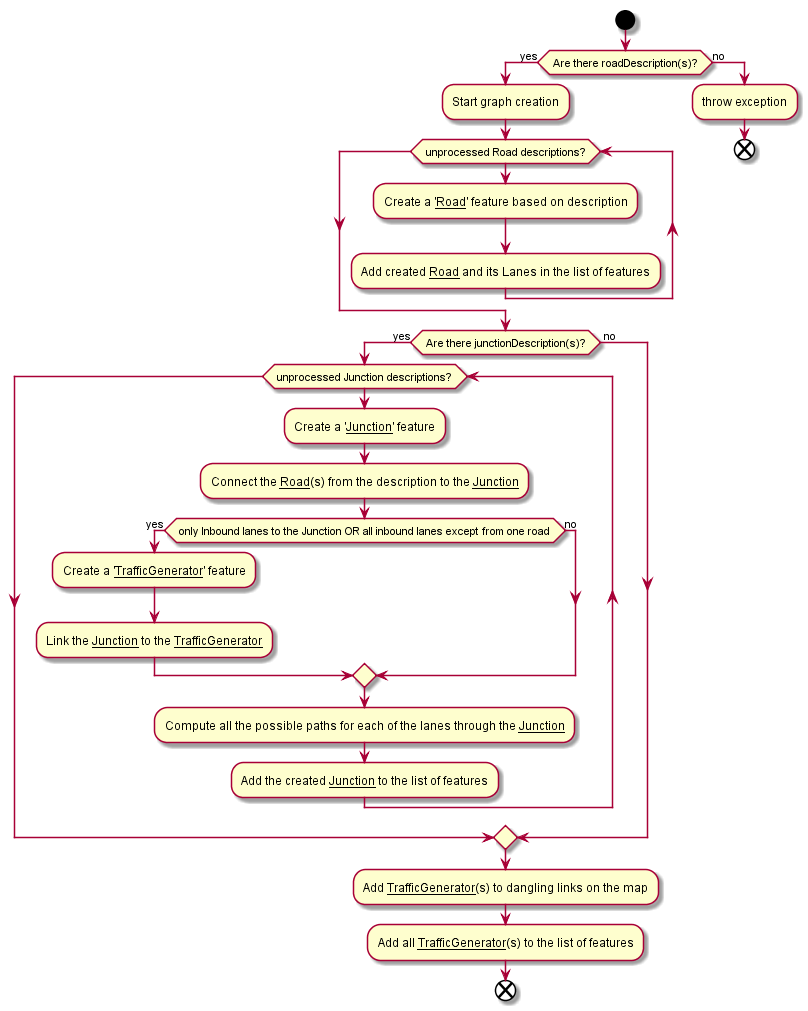
\includegraphics[width=\textwidth]{figs/graphConstruction/GraphConstruction.png}
\end{figure}

\begin{figure}[h]
  	\caption{Road construction sequence diagram}
  	\label{fig:roadConstructSeqDiag}
  	\centering
  	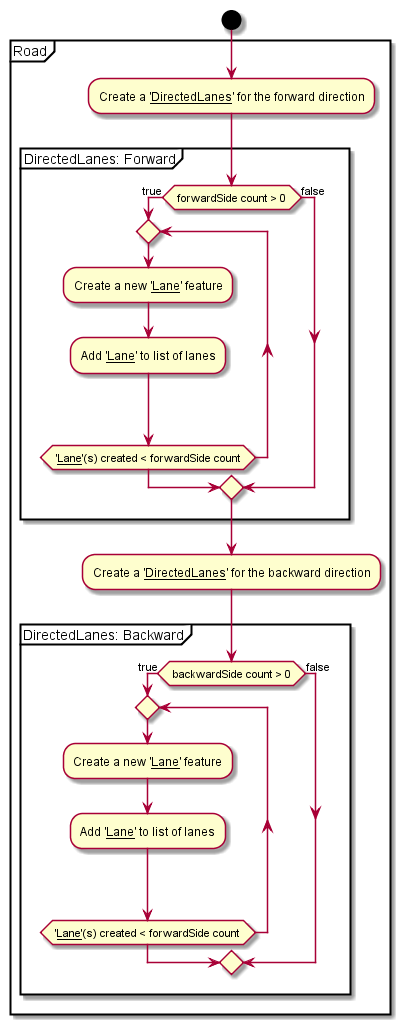
\includegraphics[width=0.45\textwidth]{figs/graphConstruction/RoadConstruction.png}
\end{figure}


\subsection{Logger}
\begin{sidewaysfigure}[h]
  	\caption{Logger class diagram}
  	\label{fig:loogerClassDiag}
  	\centering
  	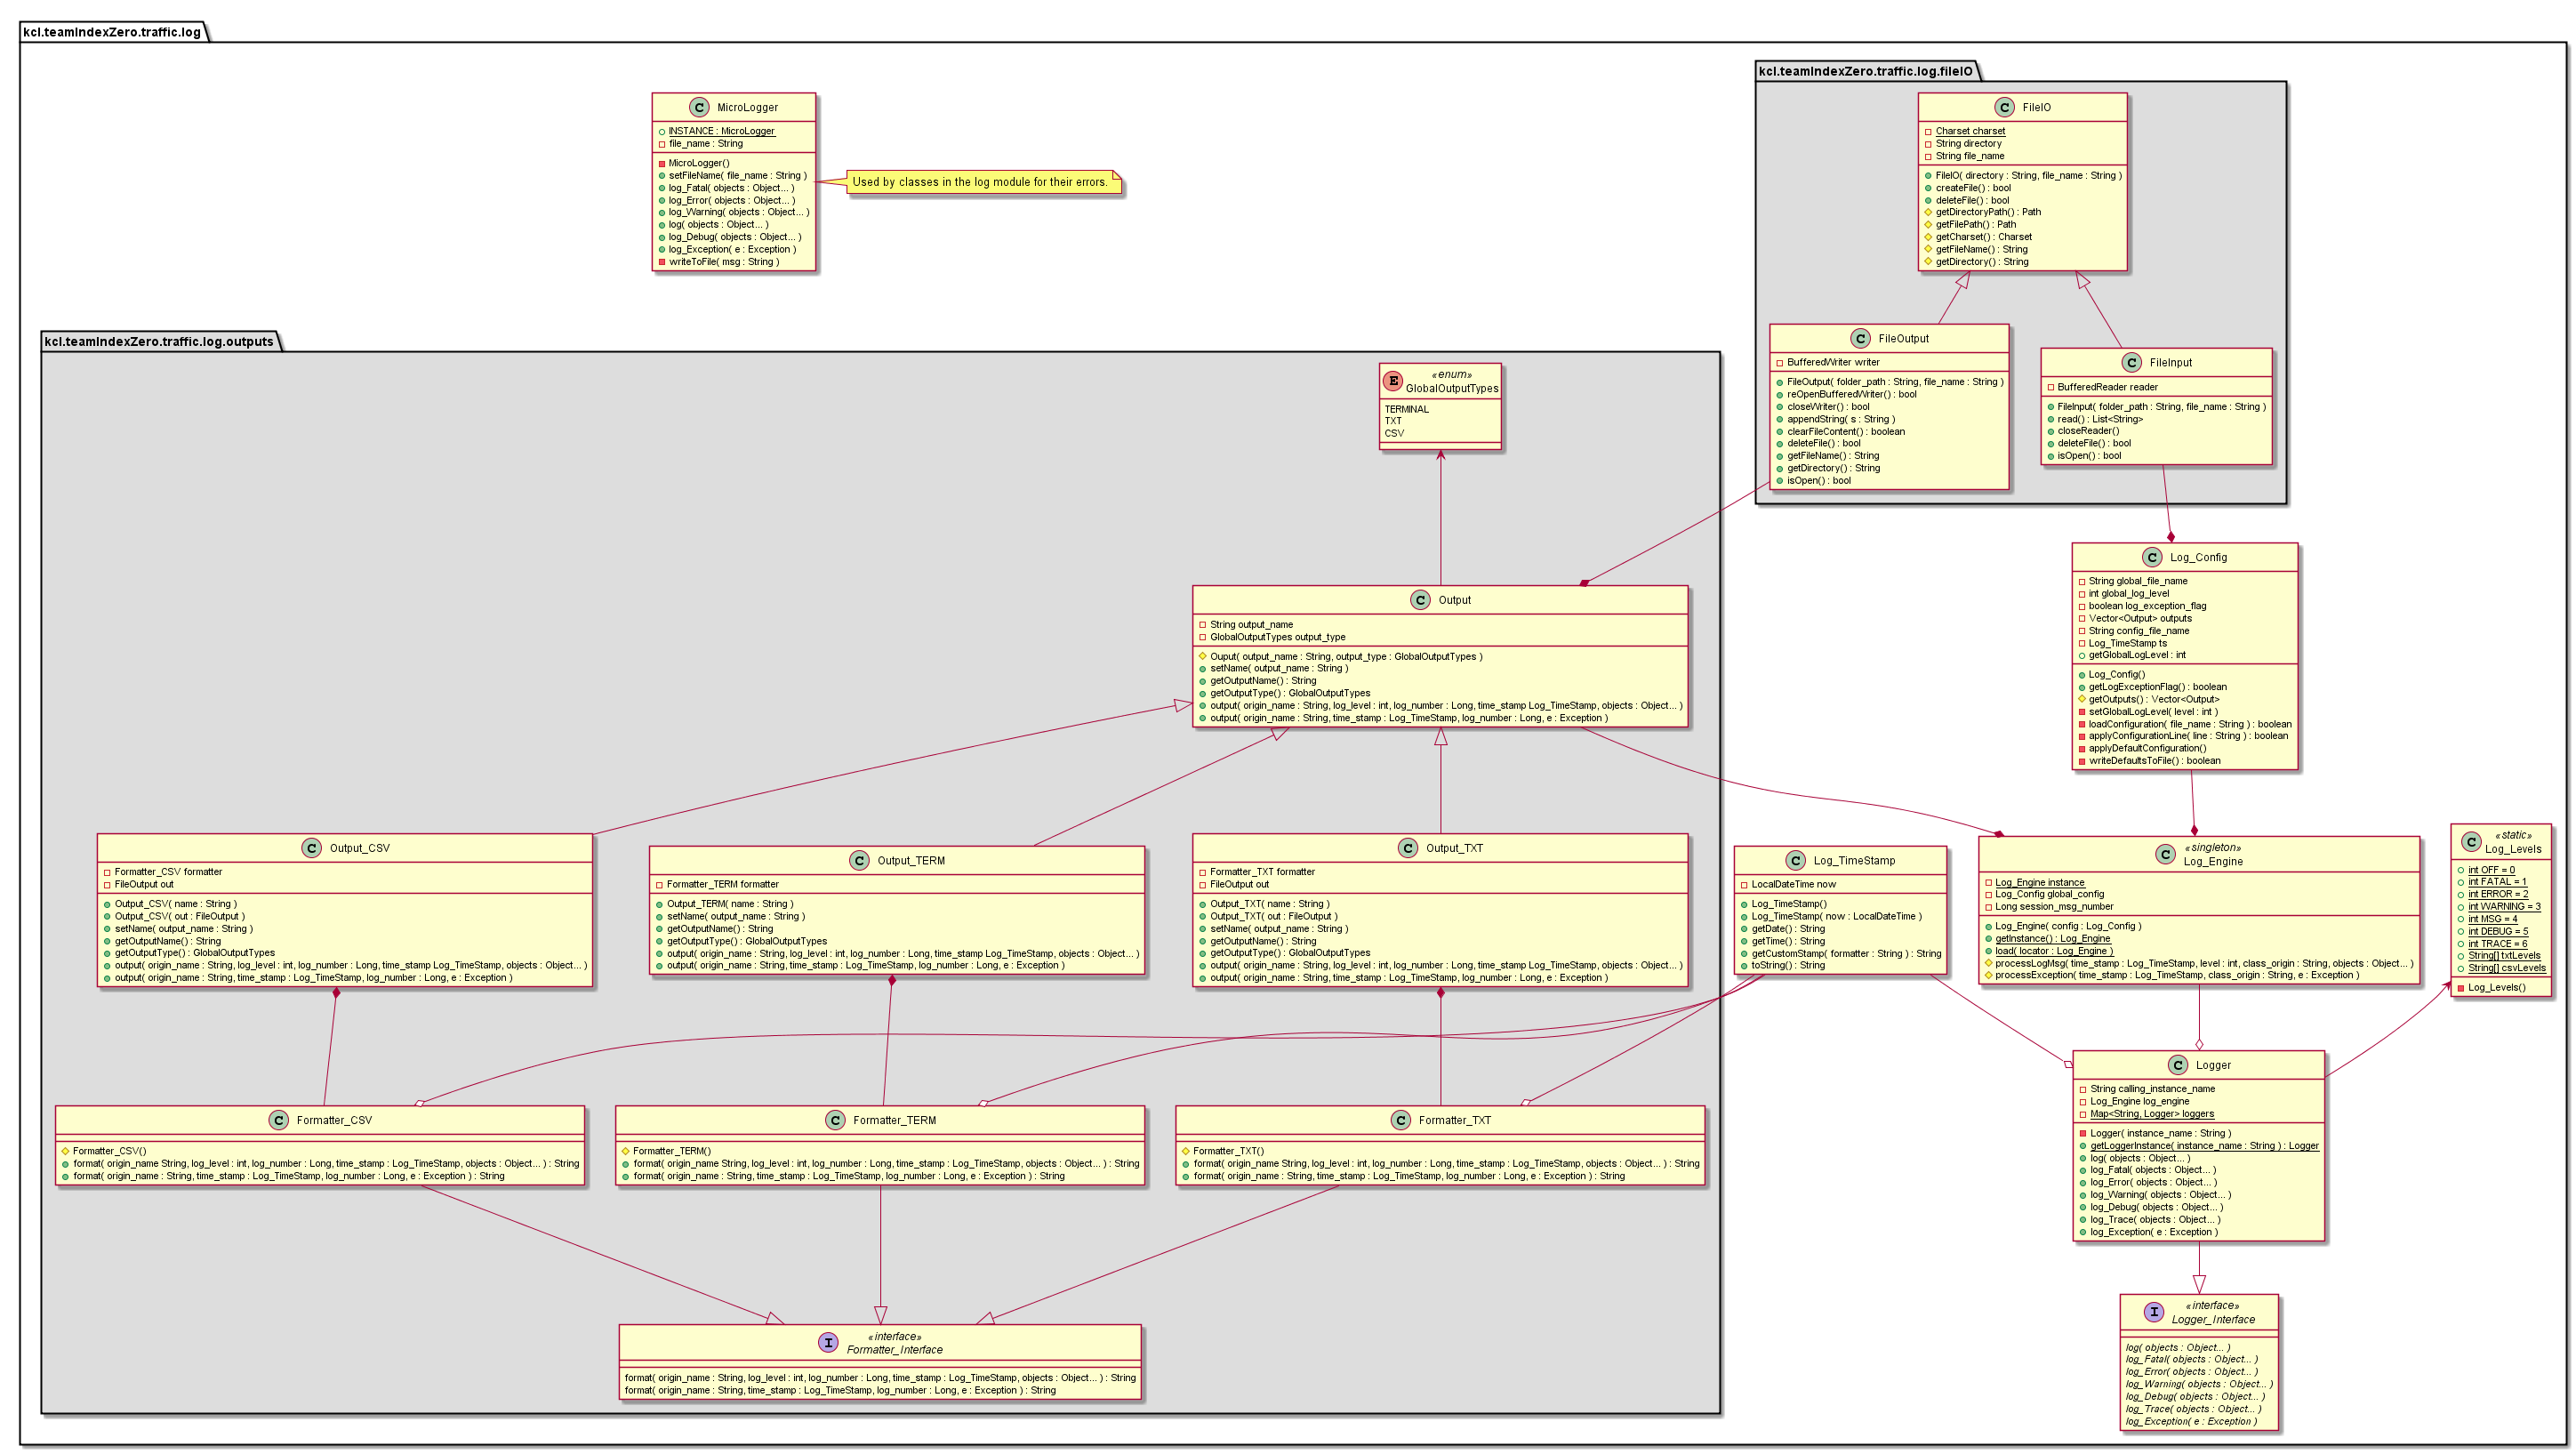
\includegraphics[width=\textheight - 2em]{figs/logger/logModuleClassDiagram.png}
\end{sidewaysfigure}
\end{document}
